\documentclass[a4paper,11pt]{article}
\usepackage[english]{babel}
\usepackage[utf8]{inputenc}
\usepackage[T1]{fontenc}
\usepackage{graphicx}
\usepackage{amsmath}
\usepackage{tikz}
\usepackage{amsthm}
\usepackage{amssymb}
\usepackage{nicefrac}
\usepackage{tabularx}
\usepackage{cprotect}
\usepackage{wrapfig}
\usepackage{framed}
\usepackage{fancyvrb}
\usepackage{bm}
\usepackage{listings}
\usepackage{longtable}
\usepackage[left=25mm,right=25mm,bottom=25mm,top=25mm]{geometry} %left, right, bottom ,top, includeheadfoot
\usepackage{caption}
\usepackage{multicol}
\usepackage{subcaption}
\usepackage{nameref}
\usepackage{placeins} %Put command \floatbarrier in front of textpassage or other items, in front of which the desired content (i.e. images) shall be placed.
\usepackage[inline]{enumitem}
% \usepackage[parfill]{parskip}
%\usepackage{fancyhdr}
\usepackage{enumitem}
\usepackage{siunitx}
\newcounter{question}
\setcounter{question}{0}
\usepackage{blindtext}
\usepackage{hyperref} %To make document linked within.
\usepackage{cleveref}
\numberwithin{equation}{section}
\captionsetup{font=footnotesize,labelfont=bf}

\renewcommand{\theenumi}{(\arabic{enumi})}
\renewcommand\labelenumi{\theenumi} % Change enumerate style from 1. to (1) etc.
\renewcommand{\theenumiii}{(\arabic{enumiii})}
\renewcommand\labelenumiii{\theenumiii} % Change enumerate style from 1. to (1) etc.
\setlist{itemsep = 0.2pt}


\newcommand\matr[1]{\ensuremath{\boldsymbol{\mathbf{#1}}}}
\newcommand\vect[1]{\ensuremath{\bm{#1}}}
\newcommand\dint{\ensuremath{\int\displaylimits}}

%\DeclareSIUnit \parsec {pc}
%\DeclareSIUnit \magnitudes {mag}
\DeclareSIUnit \curie {Ci}

\title{Machine Learning\\ \vspace{0.2cm}\normalsize Questions and Answers}
\author{Daniel Zahnd}
\date{September 16, 2024 - \today}


\newtheorem{ass}{Assertion}

\begin{document}


\newcommand\Que[1]{%
   \leavevmode\par
   \stepcounter{question}
   \noindent
   \thequestion. \textbf{Q} --- #1\par}

\newcommand\Ans[2][]{%
    \leavevmode\par\noindent
   {\leftskip0pt
    \textbf{A} --- \textbf{#1}#2\par}}

\maketitle
%\thispagestyle{empty}
\tableofcontents
%\newpage

\pagenumbering{arabic}
\setcounter{page}{1}

\section{Preliminaries}
Usually, one deals with datasets containing of data $x \in \mathbb{R}^n$ associated to other data $y$ with $n \in \mathbb{N}$. The data $x$ can be scalar of vectorial, whereas the data $y$ can also be a scalar or vector. The data $x$ is either $y \in \mathbb{R}^q$ with $q \in \mathbb{R}$ or a number of a class $\{1,\dots,K\}$ for $K \in \mathbb{N}$. In the case where e.g. $y \in \mathbb{R}$, one speaks of a regression problem, whereas in the case where $y \in\{1,\dots,K\}$ are classes, one speaks of a classification task.

Usually, one has a dataset containing of various pairs of $x$ and $y$; to distinguish an instance of data from components of a vector, one writes $(x^{(i)}, y^{(i)})$ for an instance of a dataset containing of $m \in \mathbb{N}$ instances of data. For components of an instance of data $x^{(i)} \in \mathbb{R}^n$, one writes \begin{equation}
	x^{(i)} = \begin{pmatrix}
		x^{(i)}_1 \\ \vdots \\ x^{(i)}_n
	\end{pmatrix} \in \mathbb{R}^n.
\end{equation} For a whole dataset, one can write \begin{equation}
\{(x^{(i)}, y^{(i)})\}_{i=1,\dots,m} = \{(x^{(1)}, y^{(1)}), \dots , (x^{(m)}, y^{(m)})\}.
\end{equation}

The goal in machine learning is thus to find a function $h$ with associated tunable parameters $\theta$, that predicts $y$ based on $x$; hence one can write \begin{equation}
	h_\theta(x) = y.
\end{equation} The ultimate goal usually is to determine the parameters (weights) $\theta$; whereas for the shape or nature of the function $h$, one can usually make assumptions. The $h$ is reminiscent of ``hypothesis'' and thus of ``hypothesis'' function.

\subsection{Probability measures}
\subsubsection{Random variable}
A random variable is some quantity $x$, which can take a random value. Those random values follow a certain probability distribution, which is determined by the underlying process constituting the random variable.If the probability distribution of a random variable is known, the probability density $p(x)$ can be written down for the continuous and discrete cases as \begin{equation}
	\int_{-\infty}^{\infty}p(x)\,\mathrm{d}x = 1 \qquad \text{and} \qquad \sum_{i} p(x_i) = 1.
\end{equation}

\subsubsection{Expectation value}
The expectation value $\mathbb{E}(x) \doteq \bar{x}$ of a random variable $x$ for both the continuous and discrete case is defined as \begin{equation}
	\mathbb{E}(x) = \int_{-\infty}^{\infty}xp(x)\,\mathrm{d}x \qquad \text{and} \qquad \mathbb{E}(x) = \sum_{i}x_ip(x_i).
\end{equation}

\subsubsection{Variance, standard deviation and covariance}
The variance $\mathbb{V}(x)$ of a continuous or discrete random variable $x$ can be calculated by means of \begin{equation}
	\mathbb{V}(x) = \int_{-\infty}^{\infty} (x-\bar{x})^2p(x)\,\mathrm{d}x \qquad \text{and} \qquad \mathbb{V}(x) = \sum_{i} (x_i-\bar{x})^2p(x_i).
\end{equation}
Note, that the variance $\mathbb{V}(x)$ can also be expressed as \begin{equation}\mathbb{V}(x) = \mathbb{E}\left[(x-\mathbb{E}[x])^2\right].\end{equation} The standard deviation $\sigma_x$ is defined as the square root of the variance, hence \begin{equation}
	\sigma_x = \sqrt{\mathbb{V}(x)}.
\end{equation}
Let now $x_1,\dots,x_n$ be random variables with associated probability densities $p(x_j)$, $j\in \{1,\dots,n\}$ and joint probability densities $p(x_i,x_j)$. Let furthermore be $\bar{x}_i = \mathbb{E}(x_i)$. The covariance $\mathbb{K}(x_i,x_j)$ of two random variables for the continuous and discrete case is defined as \begin{equation}\label{eq:covariance}
	\mathbb{K}(x_i,x_j) = \int_{-\infty}^{\infty}\int_{-\infty}^{\infty}(x_i-\bar{x}_i)(x_j-\bar{x}_j)p(x_i,x_j)\,\mathrm{d}x_i\,\mathrm{d}x_j
\end{equation} and \begin{equation}
	\mathbb{K}(x_i,x_j) = \sum_{k,l}(x_{i_k}-\bar{x}_i)(x_{j_l}-\bar{x}_j)p(x_{i_k},x_{j_l}).
\end{equation} Note, that the covariance $\mathbb{K}(x,y)$ of two random variables $x$ and $y$ can also be expressed as \begin{equation}\mathbb{K}(x,y) = \mathbb{E}\left[(x-\mathbb{E}[x])(y-\mathbb{E}[y])\right].\end{equation} In the context of covariance, one usually also defines the correlation coefficient $\rho(x_i,x_j)$ between two random variables as \begin{equation}\label{eq:correlationcoefficient}
	\rho(x_i,x_j) = \frac{\mathbb{K}(x_i,x_j)}{\sqrt{\mathbb{V}(x_i)\mathbb{V}(x_j)}} = \frac{\mathbb{K}(x_i,x_j)}{\sigma_{x_i}\sigma_{x_j}}.
\end{equation} % Definitions of expectation values and so on, and of Gaussian, Binomial, Poisson and Bernoulli distributions and why and when they are used

\subsection{Preliminary questions}
\Que{How is the uniform distribution defined?}
\Ans{
	Consider a continuous random variable $x$. The uniform probability distribution is defined by the probability density $p(x)$ as \begin{equation}
		p(x) = \mathcal{U}(x; a,b) = \begin{cases}
			\frac{1}{b-a} &, a \leq x \leq b \\
			0 &, \text{otherwise}
		\end{cases}
	\end{equation} where $a$ and $b$ define the domain of the distribution. The expectation value and the variance of the uniform distribution are given by \begin{equation}
		\mathbb{E}(x) = \frac{a+b}{2}, \quad \mathbb{V}(x) = \frac{1}{12}(b-a)^2.
	\end{equation} 
	
	The uniform distribution is used for processes with no prior knowledge about the probabilities of events. It is furthermore used to model processes, where all outcomes are equally likely to happen.
}

\Que{How is the standard normal distribution defined?}
\Ans{
	Consider a continuous random variable $x$. The standard normal probability distribution (Gaussian) is defined by the probability density $p(x)$ as \begin{equation}
		p(x) = \mathcal{N}(x;\mu,\sigma) = \frac{1}{\sqrt{2\pi}\sigma}e^{-\frac{(x-\mu)^2}{2\sigma^2}}
	\end{equation} where $\mu$ defines the expectation value and $\sigma$ the variance the distribution. The expectation value and the variance of the uniform distribution are given by \begin{equation}
		\mathbb{E}(x) = \mu, \quad \mathbb{V}(x) = \sigma^2.
	\end{equation} 
	
	The normal distribution is used for processes, which are influenced by an additive effect of a large number of different and independent influences modelled by arbitrary probability distributions. It pertains - with the uniform distribution - to the two default probability distributions to use, where little prior information about the modelled processes is available.
}

\Que{How is the Bernoulli distribution defined?}
\Ans{
	Consider a discrete random variable $x$. The Bernoulli probability distribution is defined by the probability density $p(x)$ as
	\begin{equation}
		p(x) = \mathcal{B}(x; p) =
		\begin{cases}
			p &, x = 1 \\
			1 - p &, x = 0 
		\end{cases},
	\end{equation}
	where $0 \leq p \leq 1$ is the probability of success (i.e., $x = 1$). The random variable $x$ takes on only two possible values: 1 (success) or 0 (failure).
	
	The expectation value and variance of the Bernoulli distribution are given by
	\begin{equation}
		\mathbb{E}(x) = p, \quad \mathbb{V}(x) = p(1 - p).
	\end{equation}
	
	The Bernoulli distribution models a single trial of an experiment where there are exactly two possible outcomes: success with probability $p$ and failure with probability $1 - p$. It is a fundamental building block of the binomial distribution, which models a sequence of independent Bernoulli trials.
}

\Que{How is the binomial distribution defined?}
\Ans{
	Consider a discrete random variable $x$. The binomial probability distribution is defined by the probability density $p(x)$ as \begin{equation}
		p(x) = \mathcal{B}(x;n,p) = \begin{cases}
			\binom{n}{x}p^x(1-p)^{n-x} &, x \in \{1,\dots,n\} \\
			0 &, \text{otherwise}
		\end{cases},
	\end{equation} where $n$ denotes the number of trials of an experiment and $p$ is the respective probability of success or failure of the outcome. The expectation value and the variance of the binomial distribution are given by \begin{equation}
		\mathbb{E}(x) = np, \quad \mathbb{V}(x) = np(1-p).
	\end{equation} 
	
	The binomial distribution is used to model processes that model a series of identical and independent experiments with exactly two possible outcomes, success or failure.
}

\Que{How is the Poisson distribution defined?}
\Ans{
	Consider a discrete random variable $x$. The Poisson probability distribution is defined by the probability density $p(x)$ as \begin{equation}
		p(x) = \mathcal{P}(x;\lambda) = \begin{cases}
			\frac{\lambda^x}{x!}e^{-\lambda} &, x \in \mathbb{N}_0 \\
			0 &, \text{otherwise}
		\end{cases},
	\end{equation} where $\lambda > 0$ defines both the expectation value and the variance. The expectation value and the variance of the Poisson distribution are given by \begin{equation}
		\mathbb{E}(x) = \lambda, \quad \mathbb{V}(x) = \lambda.
	\end{equation} 
	
	The Poisson distribution is - similarly to the binomial distribution - used to model processes that model a series of identical and independent experiments with exactly two possible outcomes, success or failure, but where the probability $p$ of success behaves as $p \rightarrow 0$ and where the number of trials $n$ behaves as $n\rightarrow \infty$.
}

\Que{How is the Poisson distribution defined?}
\Ans{
	Consider a discrete random variable $x$. The Poisson probability distribution is defined by the probability density $p(x)$ as \begin{equation}
		p(x) = \mathcal{P}(x;\lambda) = \begin{cases}
			\frac{\lambda^x}{x!}e^{-\lambda} &, x \in \mathbb{N}_0 \\
			0 &, \text{otherwise}
		\end{cases},
	\end{equation} where $\lambda > 0$ defines both the expectation value and the variance. The expectation value and the variance of the Poisson distribution are given by \begin{equation}
		\mathbb{E}(x) = \lambda, \quad \mathbb{V}(x) = \lambda.
	\end{equation} 
	
	The Poisson distribution is - similarly to the binomial distribution - used to model processes that model a series of identical and independent experiments with exactly two possible outcomes, success or failure, but where the probability $p$ of success behaves as $p \rightarrow 0$ and where the number of trials $n$ behaves as $n\rightarrow \infty$.
}

\Que{What is the popular definition of machine learning authored by Arthur Samuel in 1959?}
\Ans{According to Samuel, machine learning is the field of study that gives computers the ability to learn without being explicitly programmed. Explicitly programmed here means, that everything would be hard-coded, instead of rule-based programming.}

\Que{What is another popular definition of machine learning authored by Tom Michel in 1999?}
\Ans{
According to Michel, a well-posed machine learning problem may be described as follows: A computer program is said to learn from experience $E$ with respect to some tasks $T$ and performance measure $P$, if its performance at tasks $T$ as measured by performance $P$ improves with experience $E$.
}

\Que{Broadly speaking, which three types of machine learning algorithms are there?}
\Ans{Broadly speaking, there are three different categories of machine learning algorithms:
\begin{enumerate}
	\item Supervised learning: A machine learns how to make predictions about a specific target of interest, given some observations.
	\item Unsupervised learning: A machine learns how to find useful structures and patterns in given data by itself.
	\item Reinforcement learning: A machine has the ability to act and thus influence its own observations, thereby learning to make predictions to achieve a given goal.
\end{enumerate}

An example of supervised learning would be a classification task; that is to say to assign data to two or more given classes of objects depending on one or more variables. One could for example do this by means of linear or polynomial regression.

In comparison to supervised learning, unsupervised learning would for example try to separate data into two or more classes of objects, depending on what makes sense to the algorithm.

Reinforcement learning finally is about problems, where a sequence of decisions over time is required, where the basic idea is to implement a reward function as supervision to give the model a way to improve itself.
}

\Que{How does gradient descent work; and what is the difference between stochastic gradient descent and just gradient descent?}
\Ans{
	Gradient descent is one of the most useful and foundational techniques in machine learning; basically, it is about minimizing a loss function $J(\theta)$ with respect to weights (parameters) $\theta$ which belong to the chosen model.
	
	Hence, let now $J(\theta)$ be the loss function of a model, where $\theta = (\theta_1, \dots, \theta_n)^\top$ are the parameters of the model, which need to be optimized. The loss function might take a form as given in \cref{fig:gradientdescent}.
	\begin{figure}[h]
		\centering
		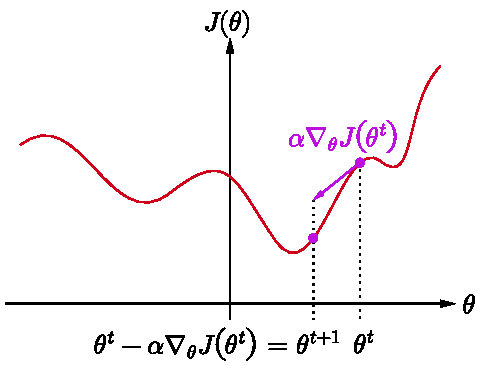
\includegraphics[width=0.4\textwidth]{figures/gradientdescent.pdf}
		\caption{Visualization of the gradient descent routine. Note, that $\theta$ is generally a vector; thus, the figure does only represent the general case in the case where $\theta$ is a scalar. If $\theta$ would consist of two components, the figure would be still visualizable in two dimensions on paper, but for higher dimensions in $\theta$, gradient descent may not be visualizable anymore on paper.}
		\label{fig:gradientdescent}
	\end{figure}
	Now, $\theta^t$ denotes the weights at iteration step $t \in \{1,\dots,T\}$ for a total iteration time $T$. Well, gradient descent updates the weights as \begin{equation}
		\theta^{t+1} = \theta^t - \alpha\nabla_\theta J(\theta^t),
	\end{equation} where the gradient is taken with respect to the weights $\theta$ and is evaluated at $\theta^t$, i.e. \begin{equation}
		\nabla_\theta = \sum_{j=1}^n e_j\partial_{\theta_j}.  \end{equation} In the case, where no confusion arises to which respect a gradient is taken, the subscript can also be left away. The parameter $\alpha$ is called the learning rate in machine learning and it has to be chosen such, that the algorithm does find the global, instead of just a local minimum of $J(\theta)$.
}

\Que{What is the rationale for the learning rate $\alpha$ in gradient descent?}
\Ans{
Consider \cref{fig:gradientdescentrationale}; it shows a curve $J(\theta)$ and a quadratic function $g(\theta) = \|\theta- \theta^t\|$. Now, one can Taylor expand the function $J(\theta)$ around
\begin{figure}[h]
	\centering
	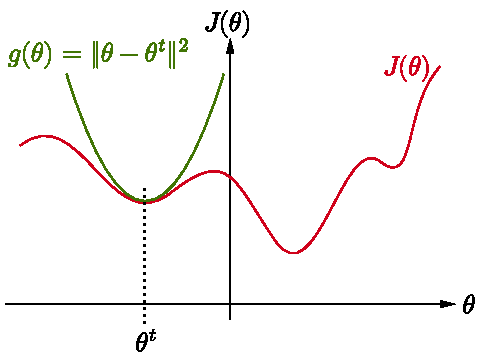
\includegraphics[width=0.4\textwidth]{figures/gradientdescentrationale.pdf}
	\caption{Rationale behind the gradient descent routine and the learning rate $\alpha$.}
	\label{fig:gradientdescentrationale}
\end{figure} % Lecture 3 about 55min in
an iteration step $\theta^t$ quite easily to first order in $\theta$ as \begin{equation}
	J(\theta) \approx J(\theta^t) + \nabla_\theta J(\theta^t)^\top (\theta - \theta^t).
\end{equation} Now, the second order term would involve the Hessian, which can be quite complicated. However, one can always add a quadratic term of the form $g(\theta)$, which is scaled by some parameter $\varepsilon$, such that the resulting approximation of $J(\theta)$ always stays above the exact function; the added term with $\varepsilon$ thus approximates the Hessian. One hence has \begin{equation}
J(\theta) \approx J(\theta^t) + \nabla_\theta J(\theta^t)^\top (\theta - \theta^t) + \frac{1}{2\varepsilon}\|\theta - \theta^t\|^2.
\end{equation} In order to find a minimum of this expression, one has to compute the gradient of the expression with respect to $\theta$, set it to zero and solve for $\theta$. From this, \begin{equation}
\nabla_\theta J(\theta) \approx 0 + \nabla_\theta J(\theta^t) + \frac{1}{\varepsilon}(\theta- \theta^t) \overset{!}{=} 0 \quad \Leftrightarrow \quad \theta = \theta^t - \varepsilon\nabla_\theta J(\theta^t)
\end{equation} follows. This is nothing but gradient descent, where $\varepsilon = \alpha$ is the learning rate. As one can see, the width $(2\varepsilon)^{-1}$ of the added quadratic term to the first order Taylor expansion of $J(\theta)$ is the inverse of the learning rate. If the learning rate is large, the width of the added quadratic term is very narrow.
}

\section{Supervised learning}
\Que{What is supervised learning? What is the goal of supervised learning?}
\Ans{
	Suppose that one has a dataset $\{(x^{(i)}, y^{(i)})\}_{i=1,\dots,m}$ of feature vector $x\in\mathbb{R}^n$ samples and associated labels $y \in\{1,\dots,K\}$. Supervised learning is about learning the parameters $\theta$ for a model that models a probability density $p(y|x; \theta)$. % Lecture 9
}
\subsection{Linear regression}
\subsubsection{Least mean squares} % Lecture 1
\Que{How can a most simple machine learning model performing affine regression be implemented?}
\Ans{
Let $x \in \mathbb{R}^n$ be a feature vector and $y \in \mathbb{R}$. Let furthermore $(x^{(i)}, y^{(i)})$ with $i \in \{1,\dots,m\}$ be a training dataset. Now, for affine regression, we can suggest a hypothesis function \begin{equation}
	h_{\theta}(x) = \theta_0 + \theta_1x_1 + \theta_2 x_2 + \dots + \theta_n x_n,
\end{equation} which, defining $x \doteq (1, x_1, x_2, \dots, x_n)^\top$, can be written more compactly as \begin{equation}
h_\theta(x) = \theta^\top x.
\end{equation} As a loss function to  minimize, it makes sense to take the Euclidean norm as a metric to measure ``closeness'' of the prediction $h_\theta(x^{(i)})$ to the actual value $y^{(i)}$, thus \begin{equation}
J(\theta) \doteq \frac{1}{2}\sum_{i=1}^{m}\|h_\theta(x^{(i)})-y^{(i)})\|^2= \frac{1}{2}\sum_{i=1}^{m}\|\theta^\top x^{(i)}-y^{(i)})\|^2.
\end{equation} The update rule for this regression task would be thus given by \begin{equation}
\theta^{t+1} = \theta^t - \alpha \nabla_\theta J(\theta) = \theta^t - \alpha \sum_{i=1}^{m}\left(\theta^\top x^{(i)}-y^{(i)}\right)x^{(i)}, 
\end{equation} where $\alpha \in \mathbb{R}$ is a suitably chosen learning rate. The proposed algorithm is called a least mean squares algorithm. This algorithm is equivalent to stating the optimal model parameters $\hat{\theta}$ as \begin{equation}
\hat{\theta} = \arg\min_\theta \left(\sum_{i=1}^m\left[\theta^\top x^{(i)}-y^{(i)}\right]^2\right).
\end{equation}
}

\Que{How can the least mean squares method be given in matrix form in the general case?}
\Ans{
Let $x \in \mathbb{R}^n$ be a feature vector and $y \in \mathbb{R}$. Let furthermore $(x^{(i)}, y^{(i)})$ with $i \in \{1,\dots,m\}$ be a training dataset. Define a matrix $X$, such that $(x^{(i)})^\top$ is the $i$-th row and a matrix $Y$, such that $y^{(i)}$ is also the $i$-th row, namely \begin{equation}
	X \doteq \begin{pmatrix}
		1 & (x^{(1)})^\top \\
		\vdots & \vdots \\
		1 & (x^{(m)})^\top
	\end{pmatrix}, \qquad Y \doteq \begin{pmatrix}
	y^{(1)} \\
	\vdots \\
	y^{(m)}
	\end{pmatrix}.
\end{equation} Hereby, a column of ones was added to the matrix $X$ to account for the shift parameter of an affine functino. Given a parameter vector $\theta^\top = (\theta_0,\theta_1,\dots,\theta_n)$, one can then write down the hypothesis function $h_\theta(X)$ as \begin{equation}
h_\theta(X) = X\theta \approx Y.
\end{equation} We thus write down the loss function as \begin{equation}
J(\theta) = \frac{1}{2}\| X\theta - Y\|^2 = \frac{1}{2}(X\theta-Y)^\top (X\theta-Y).
\end{equation} Taking the gradient $\nabla_\theta$ of this expression leads to \begin{equation}
\nabla_\theta J(\theta) = \theta^\top X^\top X - (X^\top Y)^\top.
\end{equation} Setting this expression to zero yields the closed-form solution \begin{equation}
\theta^\star = (X^\top X)^{-1}X^\top Y
\end{equation} to the optimization problem \begin{equation}
\theta^\star = \arg\min_\theta \left[J(\theta)\right].
\end{equation}
% Lecture 2
}

\Que{There is a closed form solution to the least mean squares problem? Why is it however not heavily used in practice?}
\Ans{
The reason behind this is that the closed-form solution to the least mean squares problem involves the calculation of inverse matrices. The inverse matrix to be inverted is of size $m\times m$, where $m \in \mathbb{N}$ is the amount of data instances. Calculating the inverse of a matrix is computationally very demanding, especially for large matrices, as the calculation time goes with $m^2$.

Therefore, when working with large datasets, the closed-form solution is not the best option; rather, one used the gradient descent routine, which is much more efficient with large datasets, because no inverse matrices have to be calculated.
}

\Que{How is the locally weighted affine regression method defined? What is the main difference to the normal affine regression method?}
\Ans{
Let $x \in \mathbb{R}^n$ be a feature vector and $y \in \mathbb{R}$. Let furthermore $(x^{(i)}, y^{(i)})$ with $i \in \{1,\dots,m\}$ be a training dataset. Now, the optimal parameters $\hat{\theta}$ for affine regression are found  by means of performing \begin{equation}
\hat{\theta} = \arg\min_\theta\left(\sum_{i=1}^{m}\left[\theta^\top x^{(i)}-y^{(i)}\right]^2\right).
\end{equation} Now, the locally weighted affine regression takes as an input a query vector $x$ and uses a weighting function $w_i(x)$ defined by the exponential \begin{equation}
w_i(x) = e^{-\frac{(x-x^{(i)})^2}{2\tau^2}}, \quad \tau \in \mathbb{R}
\end{equation} to weigh the samples $x^{(i)}$ close to the query more than samples further away from it. This weighting function is then multiplied by the objective, thus one has \begin{equation}
\hat{\theta} = \arg\min_\theta\left(\sum_{i=1}^{m}w_i(x)\left[\theta^\top x^{(i)}-y^{(i)}\right]^2\right)
\end{equation} for the optimal parameters $\hat{\theta}$ of the locally weighted affine regression model. Thereby, also the main difference to the normal affine regression method is evident; the locally weighted method takes as an input a query vector $x$ which requires a new optimization of the model parameters each time a new (different) query is made; the normal affine regression method however requires to find the optimal model parameters only once, independent of what the query vector $x$ will be.% Lecture 3
}

\subsubsection{Probabilistic interpretation} % Lecture 2
\Que{Which are three often used assumptions in machine learning?}
\Ans{The three main assumptions are: \begin{enumerate}
\item Feature data $x$ and associated data $y$ (related by a model $y=f(x;\theta)$) are modeled by means of a parametric probability density, that is to say, one assumes, that the data follows a probability density \begin{equation}
	p = p(y|x;\theta),
\end{equation} where $\theta$ are the model parameters.
\item The data is assumed to be independent and identically distributed (IID). This assumption allows to write a joint probability distribution $p(y^{(i)},\dots,y^{(m)}|x^{(1)},\dots,x^{(m)};\theta)$ as a simple product, namely \begin{equation}
	p(y^{(i)},\dots,y^{(m)}|x^{(1)},\dots,x^{(m)};\theta) = \prod_{i=1}^m p(y^{(i)}|x^{(i)};\theta).
\end{equation}
\item The maximum likelihood approach can be used to identify the model parameters $\theta$ for the model $y = f(x;\theta)$, that is to say the optimal model parameters are found by means of \begin{equation}
	\hat{\theta} = \arg\max_{\theta} \left(\sum_{i=1}^{m}\ln \left[p(y^{(i)}|x^{(i)};\theta) \right]\right).
	\end{equation}
\end{enumerate}}

\Que{How and under which assumptions can it be shown, that Gaussian maximum likelihood and least mean squares yield the same result?}
\Ans{Assume, that the data $y$ is given by a linear model of the feature data $x$, where Gaussian noise is added. That is to say, one has a model \begin{equation}
		y \approx h_\theta(x) = \theta^\top x + \eta, \quad p(\eta) = \mathcal{N}(\eta; \mu=0, \sigma =1).
\end{equation} The conditional probability for $y$ given $x$ can thus be written as \begin{equation}
p(y|x;\theta,\sigma)= \frac{1}{\sqrt{2\pi}\sigma}e^{-\frac{(y-\theta^\top x)^2}{2\sigma^2}},
\end{equation} where we have made the assumption that the expectation value for $y \approx h_\theta(x)$ is precisely the affine model $\theta^\top x$, thus $\mathbb{E}[h_\theta(x)]= \theta^\top x$; this is equivalent to stating, that we expect the data $y$ to follow an affine model of $x$. Now, we have samples $\{(x^{(i)},y^{(i)})\}_{i=1,\dots,m}$. The maximum likelihood approach with the given assumptions thus yields \begin{align}\begin{aligned}
p(y^{(1)},\dots,y^{(m)}|x^{(1)},\dots,x^{(m)};\theta,\sigma) = \prod_{i=1}^m p(^{(i)}|x^{(i)};\theta,\sigma)
\end{aligned}\end{align} because of the IID assumption. The optimal model parameters $\hat{\theta}$ are thus given by means of \begin{align}\begin{aligned}
\hat{\theta} &= \arg\max_{\theta,\sigma}\left(\sum_{i=1}^m\ln\left[p(y^{(i)}|x^{(i)};\theta,\sigma)\right]\right) \\
&= \arg\max_{\theta,\sigma}\left(\ln\left[\frac{1}{\sqrt{2\pi}\sigma}\right]-\frac{1}{2\sigma^2}\sum_{i=1}^{m}\left[y^{(i)}-\theta^\top x^{(i)}\right]^2\right) \\
&= \arg\min_\theta\left(\sum_{i=1}^{m}\left[\theta^\top x^{(i)}-y^{(i)}\right]^2\right),
\end{aligned}\end{align} which is exactly the equation we obtained for the affine regression model with the least squares method. Note, that in the above last step we used $\sigma =1$.
}
	
\Que{How is the maximum likelihood approach for optimization problems defined?}
\Ans{
Suppose, that one has data $y$ associated to other data $x$ by means of a model \begin{equation}
	y \approx h_\theta(x),
\end{equation} that depends on some model parameters $\theta$, which are to be found. What has to be assumed for the model $h_\theta(x)$ is that $y|x$ follows a certain probability density $p(y|x)$. Suppose now, that one has samples \begin{equation}
\{(x^{(i)}, y^{(i)})\}_{i=1,\dots,m}
\end{equation} that are independently and identically distributed, one can find the model parameters $\theta$ by means of the so-called maximum likelihood approach. One calculates \begin{align}
\begin{aligned}
	p(y^{(1)},\dots,y^{(m)}|x^{(1)},\dots,x^{(m)};\theta) = \prod_{i=1}^m p(y^{(i)}|x^{(i)};\theta).
\end{aligned}
\end{align} Hereby, the identically and independently distributed (IID) assumption has been used to write the joint probability as a product. Now, in order to find the model parameters $\theta$, this probability has to be maximized, since it should be highly likely to get precisely the samples $\{(x^{(i)}, y^{(i)})\}_{i=1,\dots,m}$. Therefore, the model parameters $\hat{\theta}$ are given by 
\begin{align}
	\begin{aligned}
		\hat{\theta} = \arg\max_{\theta} \left(\sum_{i=1}^{m}\ln \left[p(y^{(i)}|x^{(i)};\theta) \right]\right).
	\end{aligned}
\end{align} Taking the logarithm of the probability renders the product as a sum, without changing the argument of maximal probability in $\theta$.
}

\subsection{Classification and logistic regression} % Lecture 3
\Que{How is the logistic regression algorithm defined?}
\Ans{
Let $x \in \mathbb{R}^n$ be a feature vector and $y \in \{0,1\}$; this is to say, we have a binary classification task at hand. Let furthermore $(x^{(i)}, y^{(i)})$ with $i \in \{1,\dots,m\}$ be a training dataset. We want to find a model, which classifies the data $x$ into either the category $y=0$ or $y=1$. For this purpose, one can propose the hypothesis function \begin{equation}
	p(y=1|x;\theta) \approx h_\theta(x) = \frac{1}{1+e^{-\theta^\top x}}, \quad p(y=0|x;\theta) \approx 1-h_\theta(x),
\end{equation} where $\theta^\top = (\theta_0, \theta_1,\dots,\theta_n)$ and $x = (1,x_1,\dots,x_n)^\top$. Now, one can rewrite \begin{equation}
p(y=1|x;\theta) = \phi, \qquad p(y=0|x;\theta) = 1-\phi
\end{equation} and thus in general \begin{equation}
p(y|x;\theta) = \phi^y(1-\phi)^{1-y}.
\end{equation} The maximum likelihood approach now yields for the optimal model parameters $\hat{\theta}$ \begin{align}
\begin{aligned}
	\hat{\theta} &= \arg\max_\theta\left(\sum_{i=1}^{m}\ln\left[p(y^{(i)}|x^{(i)};\theta)\right]\right) \\
	&= \arg\max_{\theta}\left(\sum_{i=1}^{m}\left[y^{(i)}\ln\left(\frac{1}{1+e^{-\theta^\top x^{(i)}}}\right) + \left(1-y^{(i)}\right)\ln\left(\frac{e^{-\theta^\top x^{(i)}}}{1+e^{-\theta^\top x^{(i)}}}\right)\right]\right).
\end{aligned}
\end{align} With the resulting model, one can then query for an $x$, with which probability it belongs to the class $y=1$ or $y=0$ by means of calculating \begin{equation}
p(y=1|x;\theta) = h_\theta(x), \qquad p(y=0|x;\theta) = 1-h_\theta(x).
\end{equation}
}

\subsection{Generalized linear models} % Lecture 3, beginning at 60min in
\Que{Given some function $f(y)$ and a probability density of $y$ given by $p(y|x)$, where $x$ is some other data. What is the expectation value $\mathbb{E}[f(y)|x]$?}
\Ans{
The expectation value of a continuous random variable $y$ with probability density $p(y)$ is defined as \begin{equation}
	\mathbb{E}(y) = \int_{\mathbb{R}} y p(y)\,\mathrm{d}y.
\end{equation} Given some conditional probability density $p(y|x)$ and a function $f(y)$, the expectation value $\mathbb{E}[f(y)|x]$ is given by \begin{equation}
\mathbb{E}[f(y)|x] = \int_{\mathbb{R}} f(y) p(y|x)\,\mathrm{d}y,
\end{equation} since \begin{equation}
\int_{\mathbb{R}}p(y|x)\,\mathrm{d}y = 1  \quad \text{and} \quad \mathbb{E}[y|x] = \int_{\mathbb{R}} y p(y|x)\,\mathrm{d}y.
\end{equation}

}

\Que{What is the exponential family of probability densities and why is it important for generalized linear models?}
\Ans{
A probability density $p(y|x;\eta)$ is said to belong to the exponential family, if it can be written in the form \begin{equation}
	p(y|x;\eta) = b(y) e^{\eta^\top T(y)-a(\eta)},
\end{equation} where \begin{enumerate}
\item $\eta$ is called the natural parameter, 
\item $T(y)$ is called the sufficient statistic (oftentimes $T(y) = y$) and where
\item $a(\eta)$ is the logarithmic partition function, essentially playing the role of a normalizing constant.
\end{enumerate} Recall, that $y$ is related to $x$ by means of a hypothesis function $h_\eta(x)$; that is why $x$ appears in the conditional probability $p(y|x;\eta)$. The parameters to optimize for the family of these distributions are $\eta$.
}

\Que{What is the general framework of a generalized linear model?}
\Ans{There are three properties, by which a generalized linear model can be defined:\begin{enumerate}
		\item The parameters $\eta$ to be optimized must be of the form $\eta = \theta^\top x = \eta(\theta)$.
		\item The probability density $p(y|x;\theta)$ (where $\theta = \theta(\eta)$) used to model the data must belong to the exponential family; therefore, one has to be able to rewrite $p(y|x;\theta)$ as $p(y|x;\theta) = b(y) e^{\eta^\top T(y)-a(\eta)}$ with some $b(y)$, $T(y)$ and $a(\eta)$.
		\item The hypothesis function $h_\theta(x)$ modeling $y$ must be of the form $h_\theta(x) = \mathbb{E}(T(y)|x)$.
\end{enumerate}}

\Que{How is affine regression derived from a generalized linear model?}
\Ans{
Let $x \in \mathbb{R}^n$ be a feature vector and $y \in \mathbb{R}$. Let furthermore $(x^{(i)}, y^{(i)})$ with $i \in \{1,\dots,m\}$ be a training dataset.

In order to derive a generalized linear model, we can perform the three key steps. First, we try to choose a probability density $p(y|x)$, which is suitable for the problem and check, if the chosen density belongs to the exponential family. For the sake of simplicity, $x \in \mathbb{R}$ and $y \in \mathbb{R}$ and $\sigma = 1$ for the moment. The normal distribution reads in this case as \begin{equation}
	p(y|x;\mu) = \frac{1}{\sqrt{2\pi}}e^{-\frac{(y-\mu)^2}{2}}.
\end{equation} Rearranging terms and defining $\mu \doteq \eta$, $T(y) \doteq y$, $a(\eta) \doteq \eta^2 = \mu^2$ and $b(y) \doteq (2\pi)^{-1/2}e^{-y^2/2}$, one can rewrite the above probability density as \begin{equation}
p(y|x;\eta) = b(y) e^{\eta^\top T(y) - a(\eta)},
\end{equation} which proves that the normal distribution belongs to the exponential family. Thus, requirement (2) generalized linear (GLMs) is satisfied. Now, the third requirement of GLMs is that the hypothesis function is given by \begin{equation}
	h_\theta(x) = \mathbb{E}(T(y)|x).
\end{equation} In our case we have $T(y) = y$ and hence \begin{equation}
h_\theta(x) = \mathbb{E}(T(y)|x) = \mathbb{E}(y|x) = \int_{\mathbb{R}} y p(y|x;\eta)\,\mathrm{d}y = \eta = \mu.
\end{equation} Requirement (1) of GLMs now requires us to choose $\eta = \theta^\top x$, which gives us with $h_\theta(x) = \eta$ the hypothesis function \begin{equation}
h_\theta(x) = \theta^\top x
\end{equation} to implement, which is exactly the hypothesis function for affine regression.
}

\Que{How is logistic regression derived from a generalized linear model?}
\Ans{
Let $x \in \mathbb{R}^n$ be a feature vector and $y \in \{0,1\}$. Let furthermore $(x^{(i)}, y^{(i)})$ with $i \in \{1,\dots,m\}$ be a training dataset.

In order to derive a generalized linear model, we can perform the three key steps. First, we try to choose a probability density $p(y|x)$, which is suitable for the problem and check, if the chosen density belongs to the exponential family. We choose a Bernoulli distribution of the form \begin{equation}
	p(y|x;\phi) = \phi^y(1-\phi)^{1-y}.
\end{equation} Rearranging terms and defining $b(y) = 1$ (unity matrix), $\eta \doteq \ln\left(\frac{\phi}{1-\phi}\right)$ and $a(\eta) \doteq -\ln(1-\phi) = \ln\left(1 + e^\eta\right)$ and $T(y) \doteq y$, one can rewrite the above probability density as \begin{equation}
	p(y|x;\eta) = b(y) e^{\eta^\top T(y) - a(\eta)},
\end{equation} which proves that the Bernoulli distribution belongs to the exponential family. Thus, requirement (2) generalized linear (GLMs) is satisfied. Note, that $\eta$ relates to $\phi$ as \begin{equation}
\phi(\eta) = \frac{1}{1+e^{-\eta}}.
\end{equation} Now, the third requirement of GLMs is that the hypothesis function is given by \begin{equation}
	h_\theta(x) = \mathbb{E}(T(y)|x).
\end{equation} In our case we have $T(y) = y$ and hence \begin{equation}
	h_\theta(x) = \mathbb{E}(T(y)|x) = \mathbb{E}(y|x) = \sum_{y \in \{0,1\}} y p(y|x;\eta) = \phi.
\end{equation} Requirement (1) of GLMs now requires us to choose $\eta = \theta^\top x$, which gives us with $h_\theta(x) = \phi$ the hypothesis function \begin{equation}
	h_\theta(x) = \frac{1}{1+e^{-\theta^\top x}}
\end{equation} to implement, which is exactly the hypothesis function for logistic regression.
}

\Que{How does the perceptron connect to generalized linear models?}
\Ans{
The perceptron is nothing but a generalized linear model, if an appropriate activation function $f:\mathbb{R}^{d+1}\rightarrow \mathbb{R}$ has been chosen. Consider \cref{fig:perceptron} for a visualization.
\begin{figure}[h]
	\centering
	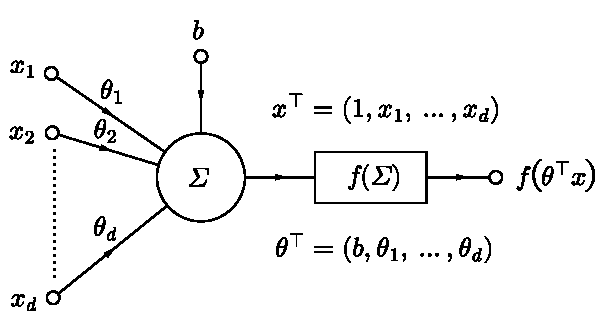
\includegraphics[width=0.5\textwidth]{figures/perceptron.pdf}
	\caption{Visualization of a basic perceptron.}
	\label{fig:perceptron}
\end{figure}  Let $x \in \mathbb{R}^d$ be a feature vector and $y \in \{0,1\}$. Let furthermore $(x^{(i)}, y^{(i)})$ with $i \in \{1,\dots,m\}$ be a training dataset. If the activation function $f$ is chosen to be the sigmoid function \begin{equation}
f(\theta^\top x) = \frac{1}{1+e^{-\theta^\top x}},
\end{equation} then, the perceptron reduces to logistic regression, as the hypothesis function in this case is \begin{equation}
h_\theta(x) = \frac{1}{1+e^{-\theta^\top x}}.
\end{equation} and hence is a form of a generalized linear model. Therefore, the perceptron with the sigmoid activation function can be trained using gradient descent as in logistic regression. This finding also generalizes; if the activation function $f$ belongs to the exponential family, every perceptron is a basic unit of a generalized linear model!
}

\Que{How is logistic regression for $k \in \mathbb{N}$ classes rather than just for two classes defined?} 
\Ans{
Logistic regression for multiple classes is also known as multinomial logistic regression or softmax regression. This is a widely used technique in machine learning to cluster data into multiple classes.
	
Softmax regression can be derived based on the framework of GLMs. Let $x \in \mathbb{R}^n$ be a feature vector and $y \in \{1,\dots,k\}$, where each index for $y$ refers to a different class. Let furthermore $(x^{(i)}, y^{(i)})$ with $i \in \{1,\dots,m\}$ be a training dataset. Now, the probability density for the multinomial case can be generalized from the binomial case, which is in that case the Bernoulli probability density. Generalized to the multinomial case, the probability density reads as \begin{equation}
	p(y|x;\theta) = \phi_1^{\mathbb{I}\{y=1\}}\cdot \dots \cdot \phi_k^{\mathbb{I}\{y=k\}},
\end{equation} where \begin{equation}
\mathbb{I}\{y=i\} = \begin{cases}
	1, \quad &y=i \\
	0, &\text{otherwise}
\end{cases}, 
\end{equation} is the indicator function and where $\phi_i = \phi_i(\theta)$ are functions of the model parameters $\theta$. One can hence write the individual probability densities $\phi_i$ as \begin{equation}
\phi_i = p(y=i|x;\theta).
\end{equation} Now, concerning the $\phi_i$, one can state that they need to add up to $1$, since this is a necessary condition on probability densities; hence we have \begin{equation}
\sum_{i=1}^{k} \phi_i = 1, \qquad \phi_k = 1-\sum_{i=1}^{k-1}\phi_i.
\end{equation} Since logistic regression is also in its multinomial form a linear model, one needs to verify the three key conditions for GLMs. First, we check, if the above proposed probability density is part of the exponential family. Towards this end, we define the function $T(y)$ as a $k-1$ dimensional vector, that for $y=i$ has a one in row $i$ but zeros in all other rows, hence \begin{equation}
[T(y)]_i = \mathbb{I}\{y=i\}, \quad i \in \{1,\dots,k-1\} \quad \Leftrightarrow \quad T(y) = \begin{pmatrix}
	\mathbb{I}\{y=1\} \\ \vdots \\ \mathbb{I}\{y=k-1\}
\end{pmatrix}.
\end{equation} With this function, we can write \begin{align}
\begin{aligned}
	p(y|x;\theta) &= \phi_1^{\mathbb{I}\{y=1\}}\cdot \dots \cdot \phi_k^{\mathbb{I}\{y=k\}} \\
	&= \phi_1^{[T(y)]_1}\cdot \dots \cdot \phi_{k-1}^{[T(y)]_{k-1}}\phi_k^{1-\sum_{j=1}^{k-1}[T(y)]_j} \\ 
	&= \exp\left([T(y)]_1\ln(\phi_1)+\dots+[T(y)]_{k-1}\ln(\phi_{k-1})+\left(1-\sum_{j=1}^{k-1}[T(y)]_j\right)\ln(\phi_k)\right) \\
	&= \exp\left([T(y)]_1\ln\left(\frac{\phi_1}{\phi_k}\right)+\dots + [T(y)]_{k-1}\ln\left(\frac{\phi_{k-1}}{\phi_k}\right)+\ln(\phi_k)\right).
\end{aligned}
\end{align} Defining a vector $\eta$ of $k-1$ elements as \begin{equation}
\eta^\top \doteq \left(\ln\left[\frac{\phi_1}{\phi_k}\right],\dots,\ln\left[\frac{\phi_{k-1}}{\phi_k}\right]\right),
\end{equation} and furthermore defining the $k$-th element as $\eta_k \doteq 0$, we can write $p(y|x;\theta)$ finally as \begin{equation}
p(y|x;\theta) = e^{\eta^\top T(y) - (-\ln[\phi_k])}.
\end{equation} If it can be shown, that $-\ln(\phi_k)$ can be written as a function $a(\eta)$ of $\eta$, it is verified that the proposed probability density $p(y|x;\theta)$ belongs to the exponential family. To this end, one calculates \begin{equation}
e^{\eta_i} = \frac{\phi_i}{\phi_k} \quad \Leftrightarrow \quad \phi_i = \phi_k e^{\eta_i}, i \in \{1,\dots,k\}.
\end{equation} Recall now, that the $\phi_i$ must sum up to 1; hence we have \begin{equation}
1=\sum_{j=1}^{k}\phi_j = \phi_k\sum_{j=1}^k e^{\eta_j} \quad \Leftrightarrow \quad  \phi_k = \frac{1}{\sum_{j=1}^k e^{\eta_j}} \quad \Leftrightarrow \quad \phi_i = \frac{e^{\eta_i}}{\sum_{j=1}^{k}e^{\eta_j}}.
\end{equation} The last expression is called the softmax function and is heavily used in deep learning as a so-called activation function for classification tasks. Assume, that a node in a deep neural network has $k$ inputs $\{\eta_1,\dots,\eta_k\}$. Acting with the softmax function on these inputs renders every input to a probability $\phi_i = e^{\eta_i}\left(\sum_{j=1}^{k}e^{\eta_j}\right)^{-1}$ of belonging to the $i$-th class. Note now, that it has been shown that $-\ln(\phi_k)$ can be written as a function of $\eta$. Hence, if $I^\top \doteq (1,\dots,1)$ is a vector of $k-1$ entries which are all ones, we can define 
\begin{equation} a(\eta) \doteq -\ln(\phi_k) = -\ln\left(\frac{1}{\sum_{j=1}^k e^{\eta_j}}\right) = -\ln\left(\frac{1}{I^\top \eta}\right).
\end{equation} Furthermore defining $b(y) = b \doteq 1$, the probability density $p(y|x;\theta)$ can indeed be written in the form \begin{equation}
p(y|x;\theta) = b(y)e^{\eta^\top T(y) - a(\eta)}
\end{equation} which proves, that said probability density belongs to the exponential family. So we can proceed with setting $\eta \doteq \theta x$, where $\theta$ now is a matrix \begin{equation}
\theta = \begin{pmatrix}
	\theta_1^\top \\ \vdots \\ \theta_{k-1}^\top
\end{pmatrix} \quad \text{such that} \quad \eta_i = \theta_i^\top x
\end{equation} consisting of vectors $\theta_1,\dots,\theta_{k-1}$, each of dimension $n$. What remains is to calculate the hypothesis function $h_\theta(x)$. So we evaluate \begin{align}
\begin{aligned}
	h_\theta(x) &= \mathbb{E}[T(y)|x] = \sum_{i=1}^{k}T(y=i) p(y=i|x;\theta)=\sum_{i=1}^k T(y=i) \phi_i = \begin{pmatrix}
		\phi_1 \\ \vdots \\ \phi_{k-1}
	\end{pmatrix}.
\end{aligned}
\end{align} For every $\phi_i$ for $i \in \{1,\dots,k-1\}$ we have \begin{equation}
\phi_i = \frac{e^{\eta_i}}{\sum_{j=1}^{k}e^{\eta_j}} = \frac{e^{\theta_i^\top x}}{1+\sum_{j=1}^{k-1}e^{\theta_j^\top x}},
\end{equation} where $\eta_k=0$ and where $\phi_k = 1-\sum_{j=1}^{k-1}\phi_j$.

So finally, one can achieve the optimal model parameters $\hat{\theta}$ by the maximum likelihood approach as \begin{align}\small
	\begin{aligned}
		\hat{\theta} &= \arg\max_\theta\left(p(y^{(1)},\dots,y^{(m)}|x^{(1)},\dots,x^{(m)};\theta)\right) \overset{\text{IID}}{=} \arg\max_\theta\left(\sum_{i=1}^{m}\ln\left[p(y^{(i)}|x^{(i)};\theta)\right]\right) \\
		&= \arg\max_\theta\left(\sum_{i=1}^{m}\ln\left[\phi_1^{\mathbb{I}\{y^{(i)}=1\}}\cdot \dots \cdot \phi_k^{\mathbb{I}\{y^{(i)}=k\}}\right]\right) \\
		&= \arg\max_\theta\left(\sum_{i=1}^{m}\sum_{j=1}^{k}\mathbb{I}\{y^{(i)}=j\}\ln(\phi_j)\right) \\
		&= \arg\max_\theta
		\left(
		\sum_{i=1}^m
		\left[
		\sum_{j=1}^{k-1}\mathbb{I}\{y^{(i)}=j\}\ln\left(\frac{e^{\theta_j^\top x^{(i)}}}{1+\sum_{l=1}^{k-1}e^{\theta_l^\top x^{(i)}}}\right)
		+
		\mathbb{I}\{y^{(i)}=k\}\ln\left(1-\sum_{u=1}^{k-1}\phi_u
		\right)
		\right]
		\right)
	\end{aligned}
\end{align} The final expression with everything plugged in reads as \begin{gather}\scriptsize\begin{gathered}
\arg\max_\theta
\left(
\sum_{i=1}^m
\left[
\sum_{j=1}^{k-1}\mathbb{I}\{y^{(i)}=j\}\ln\left(\frac{e^{\theta_j^\top x^{(i)}}}{1+\sum_{l=1}^{k-1}e^{\theta_l^\top x^{(i)}}}\right)
+
\mathbb{I}\{y^{(i)}=k\}\ln\left(1-\sum_{u=1}^{k-1}\left[\frac{e^{\theta_u^\top x^{(i)}}}{1 + \sum_{l=1}^{k-1}e^{\theta_l^\top x^{(i)}}}\right]
\right)
\right]
\right)
\end{gathered},\end{gather}
which can be maximized (or minimized with negative sign) with respect to the model parameters $\theta$.
}

\subsection{Generative learning and naive Bayes} % Lecture 4
\Que{Which are two very important formulas from probability theory heavily used in generative learning?}
\Ans{
The two formulas are the the Bayes theorem and second the marginalization theorem for probabilities.

Now, consider random variables $x$ and $y$ with probability densities $p(x)$, $p(y)$ and a joint probability density $p(x,y)$. Furthermore, conditional probabilities are given as $p(x|y)$ and $p(y|x)$. The Bayes theorem then reads \begin{equation}
	p(x|y) = \frac{p(y|x)p(x)}{p(y)} \qquad \text{or} \qquad p(y|x) = \frac{p(x|y)p(y)}{p(x)}.
\end{equation} Now, the second important formula - the marginalization theorem - is given as \begin{equation}
p(x) = \int_\mathbb{R} p(x,y)\,\mathrm{d}y \qquad \text{or} \quad p(y) = \int_{\mathbb{R}} p(x,y)\,\mathrm{d}x.
\end{equation} Now, if every event in $x$ or $y$ is disjoint from any other event possible, the law of total probability applies, which permits to write the joint probability $p(x,y)$ as \begin{equation}
p(x,y) = p(x|y)p(y) = p(y|x)p(x).
\end{equation} By means of this, the Bayes theorem can be expressed by only two assumed quantities, rather than three, namely by means of $p(x|y)$ and $p(y)$ as \begin{equation}
p(y|x) = \frac{p(x|y)p(y)}{\int_{\mathbb{R}}p(x|y)p(y)\,\mathrm{d}y},
\end{equation} where the integral discretizes to a sum, if the random variable(s) are discrete.
}

\Que{What is the difference between a discriminative and generative approach in machine learning? Explain by using the Bayes theorem!}
\Ans{
In machine learning, one models a probability density $p(y|x)$ of data $y$, given other data $x$. One can go about this using two different approaches; the generative and the discriminative approach.

The discriminative approach is to directly and explicitly define a probability density for $p(y|x)$; say, a general linear model like the logistic regression. So in this case, one has \begin{equation}
	p(y|x;\theta) = h_\theta(x),
\end{equation} where $h_\theta(x)$ is some hypothesis function like the sigmoid function, which is parametrized by model parameters $\theta$. This approach requires an explicit definition of the probability density, which is oftentimes hard to determine.

Because many times it is easier to find trustworthy expressions for the probability densities $p(x|y)$ and $p(y)$, the generative approach where one models $p(y|x)$ indirectly by means of the Bayes theorem as \begin{equation}
	p(y|x) = \frac{p(x|y)p(y)}{\int_{\mathbb{R}}p(x|y)p(y)\,\mathrm{d}y}
\end{equation} is easier. This is also the difference between the two approaches; the discriminative approach models $p(y|x)$ explicitly, whereas the generative approach models $p(y|x)$ indirectly by means of modeling $p(x|y)$ and $p(y)$ and applying the Bayes theorem.
}

\Que{What is generative learning?}
\Ans{Oftentimes, one wants to model the probability density $p(y|x)$, where $x = (x_1,\dots,x_n)^\top$ for example contain variables like the amount of rooms and the total living area of a house, and where $y$ would denote the prize of the house. This is called discriminative learning; so one wants to infer primarily one variable based on other variables.

The other way round, where one models $p(x|y)$, is called generative learning. There, one wants to infer more than one variables based on one variable. For example, one wants to have probability densities for the amount of rooms and the total living area of a house, if one only knows the probability density for the prize.}

\Que{How does Gaussian discriminative analysis (GDA) work?}
\Ans{Gaussian discriminative analysis is an example of a generative learning model. Hence, we assume the probabilities $p(x|y)$ and $p(y)$ in order to calculate $p(y|x)$ via the Bayes theorem. 
	
Let $y$ be a variable that can take two values; either $0$ or $1$. Thus, the probability $p(y;\phi)$ can be given by a Bernoulli probability density as $p(y=1;\phi) = \phi$ and $p(y=0;\phi) = 1-\phi$, where $\phi \in [0,1]$. For the probabilities $p(x|y=0;\mu_0, \Sigma)$ and $p(x|y=1;\mu_0;\Sigma)$, we assume Gaussian probability densities; thus one can write \begin{align}
	\begin{aligned}
		p(x|y=0;\mu_0,\Sigma) = \mathcal{N}(x; \mu_0, \Sigma), \quad p(x|y=1;\mu_0, \Sigma) = \mathcal{N}(x; \mu_1, \Sigma),
	\end{aligned}
	\end{align} where \begin{equation}
	\mathcal{N}(x; \mu, \Sigma) = \frac{1}{(2\pi)^{n/2}|\Sigma|^{1/2}}\exp\left(-\frac{1}{2}(x-\mu)^\top \Sigma^{-1}(x-\mu)\right)
\end{equation} is the $n$-dimensional multivariate normal distribution, where $\Sigma$ is the covariance matrix of the different components $x = (x_1,\dots,x_n)^\top$ and $\mu = (\mu_1,\dots,\mu_n)^\top$ is a vector of mean values for each component. The expression $|\Sigma|$ means $|\Sigma| = \det(\Sigma)$. Note, that the covariance matrix is assumed to be the same for both probability densities above, but not the mean values. In one expression, $p(x|y)$ and $p(y)$ can be written as \begin{align}\begin{aligned}
p(x|y;\mu_0,\mu_1,\Sigma) = \frac{1}{(2\pi)^{n/2}|\Sigma|^{1/2}}\prod_{j=0}^{1}\exp\left(-\frac{1}{2}(x-\mu_j)^\top \Sigma^{-1}(x-\mu_j)\right)^{\mathbb{I}\{y=j\}}
\end{aligned}\end{align} and \begin{equation}
p(y;\phi) = \phi^{\mathbb{I}\{y=1\}}(1-\phi)^{\mathbb{I}\{y=0\}}.
\end{equation}

The model parameters $\theta$ to learn by optimization are therefore given by \begin{equation}
	\theta= \{\mu_0, \mu_1, \Sigma, \phi\}.
\end{equation} Let $x \in \mathbb{R}^n$ be a feature vector and $y \in \{0,1\}$. Let furthermore $(x^{(i)}, y^{(i)})$ with $i \in \{1,\dots,m\}$ be a training dataset. The way to go about optimization is taking the maximum likelihood of the data; thus we want to maximize $L(\theta) \doteq \sum_{i=1}^m p(y^{(i)}|x^{(i)};\theta)$ with respect to $\theta$. This is equivalent to the formulation \begin{align} \begin{aligned}
\hat{\theta} &= \arg\min_\theta\left[l(\theta)\right] = \arg\min_\theta\left(\overbrace{-\sum_{i=1}^{m}\ln\left[p(x^{(i)}|y^{(i)};\theta)p(y^{(i);\theta})\right]}^{\doteq\,l(\theta)}\right) \\ &= \arg\min_\theta\left(-\sum_{i=1}^{m}\ln\left[p(x^{(i)}|y^{(i)};\theta)\right] - \sum_{i=1}^{m}\ln\left[p(y^{(i)};\theta)\right]\right)
\end{aligned}\end{align} for the optimal model parameters $\hat{\theta}$. Now, explicitly inserting the probability densities, one obtains \begin{align}\scriptsize
\begin{aligned}
	\hat{\theta} = \arg\min_\theta\left(\sum_{i=1}^{m}\left[\frac{1}{2}\ln\left(|\Sigma|\right) - \mathbb{I}\{y^{(i)}=0\}\left(f(x^{(i)}, \mu_0, \Sigma)+\ln(1-\phi)\right) - \mathbb{I}\{y^{(i)}=1\}\left(f(x^{(i)}, \mu_1, \Sigma)+\ln(\phi)\right)\right]\right),
\end{aligned}
\end{align} where $f(x^{(i)}, \mu_j, \Sigma) \doteq \frac{1}{2}(x^{(i)}-\mu_j)^\top \Sigma^{-1}(x^{(i)}-\mu_j)$ was defined. Now, the expression $l(\theta)$ can be optimized with respect to every model parameter $\theta= \{\mu_0,\mu_1,\Sigma, \phi\}$ by means of calculating the partial derivative with respect to every parameter, setting it to zero and solving for the parameter. Thus, one obtains \begin{align}\small
\begin{aligned}
	\phi &= \frac{1}{m}\sum_{i=1}^m\mathbb{I}\{y^{(i)}=1\}, \\
	\mu_0 &= \frac{\sum_{i=1}^{m}\mathbb{I}\{y^{(i)}=0\}x^{(i)}}{\sum_{i=1}^{m}\mathbb{I}\{y^{(i)}=0\}}, \\
	\mu_1 &= \frac{\sum_{i=1}^{m}\mathbb{I}\{y^{(i)}=1\}x^{(i)}}{\sum_{i=1}^{m}\mathbb{I}\{y^{(i)}=1\}}, \\
	\Sigma &= \frac{1}{m}\left(\mathbb{I}\{y^{(i)}=0\}\sum_{i=1}^{m}(x^{(i)}-\mu_0)(x^{(i)}-\mu_0)^\top+   \mathbb{I}\{y^{(i)}=1\}\sum_{i=1}^{m}(x^{(i)}-\mu_1)(x^{(i)}-\mu_1)^\top\right).
\end{aligned} 
\end{align} After finding the optimal parameters $\hat{\theta} = \{\hat{\mu}_0, \hat{\mu}_1, \hat{\Sigma}, \hat{\phi}\}$, one can then make a classification of a new sample $x^{(s)}$ by means of calculating
\begin{align}\begin{aligned}
	p(y=1|x^{(s)};\hat{\theta}) &= p(x^{(s)}|y=1; \hat{\theta})p(y=1;\hat{\theta}) \\
	&=\frac{\hat{\phi}}{(2\pi)^{n/2}|\hat{\Sigma}|^{1/2}}\exp\left({-\frac{(x^{(s)}-\hat{\mu}_1)^\top \hat{\Sigma}^{-1}(x^{(s)}-\hat{\mu}_1)}{2}}\right).
\end{aligned}\end{align} If $p(y=1|x^{(s)};\hat{\theta}) > 0.5$ for a sample $x^{(s)}$, then $x^{(s)}$ belongs to class 1, whereas otherwise $x^{(s)}$ belongs to class 0.

Note, that $p(y=1|x^{(s)};\theta)$ can be written as a sigmoid function with an appropriate $\theta$, which is a function of the parameters $\mu_0$,$\mu_1$, $\Sigma$ and $\phi$. Therefore, the Gaussian discriminative analysis (GDA) is very similar to logistic regression, makes however stronger assumptions. Therefore, GDA is better than logistic regression, where the GDA assumptions are fullfilled, but if that is not the case, logistic regression will yield better results.
}

\Que{How does the naive Bayes approach work?}
\Ans{Consider a problem where one has a vector $x = (x_1,\dots,x_n)^\top \in \mathbb{R}^n$ of zeros and ones. Such a vector could for example contain a one at $x_j$, if the $j$-th word of a dictionary containing $n$ words is in a checked text; say, for a spam/non-spam classification. Correspondingly, one has a class label $y \in \{1,\dots,K\}$ for $K$ classes; for example $K=1$ could denote work-related mails, $K=2$ spam and so on. Suppose furthermore, that one has at disposal a training dataset $\{(x^{(i)}, y^{(i)})\}_{i=1,\dots,m}$.
	
In this case, a naive Bayes algorithm can be applied. It is an example of a generative approach; thus we model $p(y|x;\theta)$ based on the Bayes theorem \begin{equation}
	p(y|x;\theta) \propto p(x|y;\theta)p(y;\theta),
\end{equation} where $\theta$ are the model parameters of the naive Bayes classifier. Suppose, that we have a weights vector $\theta = (\phi_{1|y=1},\dots,\phi_{1|y=K},\dots,\phi_{n|y=1},\dots,\phi_{n|y=K},\phi_{y=1},\dots,\phi_{y=K})^\top$ containing $N = nK + K = K(n+1)$ weights. If one has for example $n=9999$ words in a dictionary and $K=10$ classes to classify incoming emails, one would have $N=K(n+1) = 10(9999+1) = 10^5$ model parameters.

Now, the probability $p(x_i = 1|y=k)$ that an object contains element $i$, given that it belongs to class $k$, can be given by $p(x_i=1|y=k;\theta) = \phi_{i|y=k}$. Correspondingly, the probability $p(x_i=0|y=k;\theta)$ must be given as $p(x_i=0|y=k;\theta) = 1-\phi_{i|y=k}$. Furthermore, the probability $p(y=k;\theta)$ that an object belongs to class $k$ is given by $p(y=k;\theta) = \phi_{y=k}$. Written as sole expressions, the probabilities $p(x_i|y;\theta)$ and $p(y;\theta)$ can be given as \begin{align}
	\begin{aligned}
		p(x_i|y;\theta) = \prod_{j=1}^{K}\phi_{i|y=j}^{\mathbb{I}\{x_i=1, y=j\}}(1-\phi_{i|y=j})^{\mathbb{I}\{x_i=0, y=j\}}, \qquad
		p(y;\theta) = \prod_{j=1}^{K}\phi_{y=j}^{\mathbb{I}\{y=j\}}.
	\end{aligned}
\end{align} The naive Bayes assumption is that the events $x_i|y=k$ and $x_j|y=k$ are independent of one another for any $i,y\in\{1,\dots,n\}$ and $k\in\{1,\dots,K\}$. This allows us to write $p(x|y; \theta) = p(x_1,\dots,x_n|y;\theta) = \prod_{i=1}^{n}p(x_i|y;\theta)$. Thus, we have \begin{equation}
p(y|x;\theta) \propto p(x|y;\theta)p(y;\theta) = \prod_{i=1}^{n}\prod_{j=1}^{K}\phi_{y=j}^{\mathbb{I}\{y=j\}}\phi_{i|y=j}^{\mathbb{I}\{x_i=1, y=j\}}(1-\phi_{i|y=j})^{\mathbb{I}\{x_i=0, y=j\}}.
\end{equation} The expression, one would like to maximize, is \begin{equation}
L(\theta) = \sum_{i=1}^{m}p(y^{(i)}|x^{(i)};\theta).
\end{equation} This is equivalent to minimizing the log-likelihood $l(\theta) \doteq - \sum_{k=1}^{m}\ln\left[p(y^{(i)}|x^{(i)};\theta)\right]$ as \begin{align}\tiny\begin{aligned}
l(\theta) = -\sum_{k=1}^{m}\sum_{i=1}^{n}\sum_{j=1}^{K}\left[\mathbb{I}\{y^{(k)}=j\}\ln\left(\phi_{y=j}\right) + \mathbb{I}\{x_i^{(k)}=1,y^{(k)}=j\}\ln\left(\phi_{i|y=j}\right)+ \mathbb{I}\{x_i^{(k)}=0,y^{(k)}=j\}\ln\left(1-\phi_{i|y=j}\right)\right].
\end{aligned}\end{align} Calculating the derivatives with respect to all model parameters contained in $\theta$, setting the derivatives to zero and solving for the parameter, one would obtain the optimal model parameters $\hat{\theta}$.

We now consider a case, where we have only two classes $y\in\{0,1\}$. In that case, the log-likelihood to minimize simplifies to \begin{align}\footnotesize\begin{aligned}
		l(\theta) &= -\sum_{k=1}^{m}\sum_{i=1}^{n}\sum_{j=0}^{1}\left[ \mathbb{I}\{x_i^{(k)}=1,y^{(k)}=j\}\ln\left(\phi_{i|y=j}\right)+ \mathbb{I}\{x_i^{(k)}=0,y^{(k)}=j\}\ln\left(1-\phi_{i|y=j}\right)\right] \\
		&\quad\ -\sum_{k=1}^{m}\left[\mathbb{I}\{y^{(k)}=0\}\ln\left(\phi_y\right) + \mathbb{I}\{y^{(k)}=1\}\ln\left(1-\phi_y\right)\right],
\end{aligned}\end{align} where $\phi_{y=0} \doteq \phi_y$ was redefined. Minimizing $l(\theta)$ leads to the optimal model parameters $$\hat{\theta} = (\hat{\phi}_{1|y=0},\dots,\hat{\phi}_{n|y=0},\hat{\phi}_{1|y=1},\dots,\hat{\phi}_{n|y=1},\hat{\phi}_y)^\top$$ as \begin{align}
\begin{aligned}
	\hat{\phi}_{i|y=0} &= \frac{\sum_{k=1}^m \mathbb{I}\{x_i^{(k)}= 1, y^{(k)}=0,\}}{\sum_{k=1}^{m}\mathbb{I}\{y^{(k)}=0\}}, \\
	\hat{\phi}_{i|y=1} &= \frac{\sum_{k=1}^m \mathbb{I}\{x_i^{(k)}= 1, y^{(k)}=1,\}}{\sum_{k=1}^{m}\mathbb{I}\{y^{(k)}=1\}}, \\
	\hat{\phi}_y &= \frac{\sum_{k=1}^{m}\mathbb{I}\{y^{(k)}=0\}}{m}.
\end{aligned}
\end{align} Now that the optimal model parameters are known, one can make a prediction on a new sample $x^{(s)}$ whether it belongs to class $y=0$ or class $y=1$ by means of calculating \begin{align}\footnotesize\begin{aligned}
p(y=1|x^{(s)};\hat{\theta}) = \frac{p(x^{(s)}|y=1;\hat{\theta})p(y=1;\hat{\theta})}{p(x^{(s)};\hat{\theta})}= \frac{p(x^{(s)}|y=1;\hat{\theta})p(y=1;\hat{\theta})}{p(x^{(s)}|y=1;\hat{\theta})p(y=1;\hat{\theta}) + p(x^{(s)}|y=0;\hat{\theta})p(y=0;\hat{\theta})}.
\end{aligned}\end{align} If $p(y=1|x^{(s)};\hat{\theta}) > 0.5$, then $x^{(s)}$ belongs to class $y=1$; if not, $x^{(s)}$ belongs to class $y=0$.
}

\Que{What is Laplace smoothing in the context of the naive Bayes approach?}
\Ans{
Consider a random variable $z$ taking values $\{1,\dots,k\}$. One can parametrize this using probabilities $\phi_i = p(z=i)$. Given a set of $m$ independent observations $\{z^{(1)},\dots,z^{(m)}\}$, the maximum likelihood estimates $\hat{\phi}_j$ for this case are then derived to be \begin{equation}
	\hat{\phi}_j = \frac{\sum_{i=1}^{m}\mathbb{I}\{z^{(i)}=j\}}{m}.
\end{equation} If the training dataset however does not contain a single instance where $z = l$ for example, the corresponding probability $\phi_l$ will be estimated as zero, leading to a decision problem for the model, because both nominator and denominator of the Bayes theorem to generate the posterior will be zero.

This problem can be solved by so-called Laplace smoothing. One just adds to the maximum likelihood estimators $+1$ in the nominator, and $+k$ in the denominator, where $k$ is the number of possible values for $z$. Therefore, the modified maximum likelihood estimators will be given as \begin{equation}
	\hat{\phi}_j = \frac{\sum_{i=1}^{m}\mathbb{I}\{z^{(i)}=j\}+1}{m+k}.
\end{equation} It can be shown, that these are still valid probailities, as \begin{align}
\begin{aligned}
	\sum_{j=1}^{k}\hat{\phi}_j &= \sum_{j=1}^{k}\left(\frac{\sum_{i=1}^{m}\mathbb{I}\{z^{(i)}=j\}+1}{m+k}\right) = \frac{1}{m+k}\sum_{j=1}^{k}\left(\sum_{i=1}^{m}\mathbb{I}\{z^{(i)}=j\}+1\right) \\
	&= \frac{1}{m+k}\left(k + \underbrace{\sum_{i=1}^{m}\mathbb{I}\{z^{(i)}=1\} + \dots + \sum_{i=1}^{m}\mathbb{I}\{z^{(i)}=k\}}_{=\,m} \right) = 1
\end{aligned}
\end{align} shows. Notice, that if the value $z=l$ never occurs in the training dataset, the probability $\phi_l$ will be estimated as $\phi_l = 1/(m+k)$; the most unlikely, but not impossible event.
}

%\Que{How does the multinomial event model work?}
%\Ans{
%Text.
%}

\subsection{Support vector machines} % Lectures 4 and 5
\Que{What is the general idea behind support vector machines?}
\Ans{Let $x \in \mathbb{R}^n$ be a feature vector and $y \in \{-1,1\}$. Let furthermore $(x^{(i)}, y^{(i)})$ with $i \in \{1,\dots,m\}$ be a training dataset.
 
Now, the idea of a support vector machine is that one tries to find a hyperplane (dimension $\mathbb{R}^{n-1}$) in the feature space ($\mathbb{R}^n$), that separates positives ($y=+1$) from negatives ($y=-1$). That means, we have a classifier \begin{equation}
	h_{w,b}(x) = g(w^\top x + b), \qquad g(z) = \begin{cases}
		1, \quad &z \geq 0 \\
		0, \quad &z < 0
	\end{cases},
\end{equation} where $w$ is a vector and $b$ a scalar; $w$ and $b$ comprise the model parameters of the support vector machine. The separating hyperplane between positives and negatives is given by the equation $w^\top x + b = 0$. Graphically, one can depict this a seen in \cref{fig:scheme_svm}.
\begin{figure}[h]
	\centering
	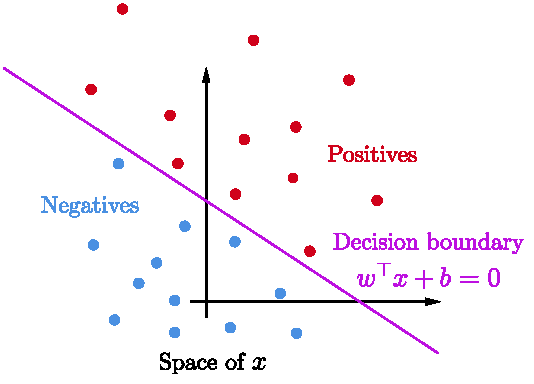
\includegraphics[width=0.4\textwidth]{figures/scheme_svm.pdf}
	\caption{Schematic view of the working principle of a support vector machine.}
	\label{fig:scheme_svm}
\end{figure}
}

\Que{Where does the name ``support vector machine'' come from?}
\Ans{
The term ``vector'' comes from the inputs $x$, which are to be classified to belong either to the class $y=-1$ (negatives) or to the class $y=+1$ (positives). As a matter of fact, mostly the samples $x^{(i)}$ closest to the decision boundary actually decide on the location of it; only those vectors support the decision on the decision boundary - this is where the term ``support'' comes from.}

\Que{What are the geometrical and functional margins with respect to the support vector machines (SVMs)? Why are both functional aswell as geometrical margin necessary?}
\Ans{
	In SVMs, the decision boundary for the SVM to decide if a new sample $x^{(j)}$ belongs to the category $y=+1$ or $y=-1$ is given by $w^\top x + b=0$, where $w$ is a vector and $b$ a scalar. All vectors $x$ that fulfill this condition live on the decision boundary (hyperplane). If the new sample $x^{(j)}$ however is not part of the decision hyperplane, then the quantity $w^\top x + b$ will either be a positive or a negative number. If it is a negative number, $x^{(j)}$ will belong to the negatives, while if it is positive, it will belong to the positives, so we have \begin{equation}
		w^\top x^{(j)}+b \geq 0 \quad \Rightarrow \quad y^{(j)} =1, \qquad w^\top x^{(j)} + b < 0 \quad \Rightarrow \quad y^{(j)} = -1.
	\end{equation} Thus one can make the number $w^\top x^{(j)} + b$ positive for any sample by means of defining the functional margin $\tilde{\gamma}^{(j)}$ for a particular sample as \begin{equation}
	\tilde{\gamma}^{(j)} = y^{(j)}\left(w^\top x^{(j)}+ b\right).
	\end{equation} The functional margin gives a metric of distance of a sample $x^{(j)}$ from the decision hyperplane and thus is a measure on the confidence of the decision; if the functional margin for a sample is very large, the decision to which class it belongs will be a confident one. However, the functional margin definition is insensitive to scaling factors; therefore, the definition of an alternative margin - the so-called geometrical margin - is necessary. The minimal functional margin $\tilde{\gamma}$ is given by \begin{equation}
	\tilde{\gamma} = \min_{j=1,\dots,m}\tilde{\gamma}^{(j)}
	\end{equation} for a set of $m$ training samples.
	
	Consider \cref{fig:geometrical_margin} for a visualization of the meaning of the geometrical margin. The weights vector $w$ is always orthogonal to the decision boundary, as $w\cdot \left(w^\top x + b\right) = 0$ for any $x$ on the decision boundary. Hence, one can measure the distance of a sample $x^{(i)}$ from the decision boundary along $w$. For any $x^{(i)}$, one can hence write $w^\top \left(x^{(i)} - \alpha^{(i)}w\right) + b = 0$, where $\alpha^{(i)}$ is a scalar needed to scale $w$ appropriately to obtain the orthogonal distance of $x^{(i)}$ to the decision boundary. Solving for $\alpha^{(i)}$ yields \begin{equation}
		\alpha^{(i)} = \frac{w^\top x^{(i)}+ b}{\|w\|^2}.
	\end{equation}
	\begin{figure}[h]
		\centering
		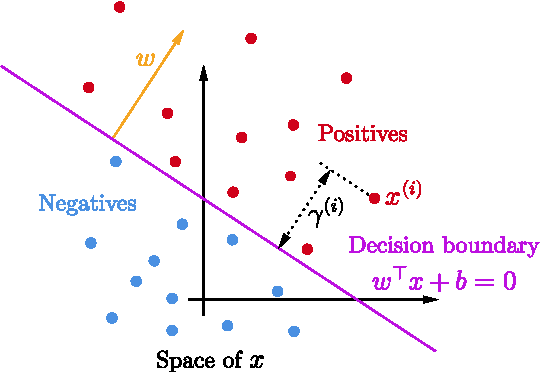
\includegraphics[width=0.4\textwidth]{figures/geometrical_margin.pdf}
		\caption{Visualization of the construction of the geometrical margin in SVMs.}
		\label{fig:geometrical_margin}
	\end{figure} The geometric margin $\gamma^{(j)}$ for any sample $x^{(j)}$ as the positive orthogonal distance of the sample from the boundary hyperplane can therefore be defined as \begin{equation}
	\gamma^{(j)} = y^{(j)}\alpha^{(j)}\|w\| = \left(\frac{w^\top x^{(j)}}{\|w\|}+\frac{b}{\|w\|}\right)y^{(j)}.
	\end{equation} The minimal geometric margin $\gamma$ is accordingly defined by \begin{equation}
	\gamma = \min_{j=1,\dots,m} \gamma^{(j)}.
	\end{equation} Note, that in the case of $\|w\| = 1$, functional and geometric margin are identical.
	
	The reason why both functional and geometric margin are defined is because only one of them is sensitive to the actual distance of a sample from the decision boundary.
}

\Que{How is a support vector machine mathematically described?}
\Ans{
Mathematically speaking, a support vector machine is all about tuning the model parameters $w$ and $b$ such that the minimum geometric margin is maximized for the training dataset. That is, if one has a dataset of $m$ pairs of $x^{(i)}$ and $y^{(i)}$, then the optimal model parameters $w^*$ and $b^*$ need to be chosen such that
\begin{equation}
	w^*, b^* \quad \text{such that} \quad \max_{w,b}\left(\min_{w,b,i=1,\dots,m}\left[\gamma^{(i)}\right]\right).
\end{equation}

The easiest way to define the optimization problem would be to require \begin{equation}
	\max_{w, b}\left(\gamma\right) \quad \text{such that} \quad y^{(i)}\left(w^\top x^{(i)} + b\right) \geq \gamma \quad  \forall i = 1,\dots,m, \quad \|w\|=1.
\end{equation} Here, the geometric margin is maximized, whereas the condition $\|w\|=1$ ensures that the geometric margin is identical to the functional margin. This ensures, that both functional and geometric margin are maximized. Because functional and geometric margin are related as $\gamma = \tilde{\gamma}/\|w\|$, one can also formulate the optimization problem as 
\begin{equation}
	\max_{w, b}\left(\frac{\tilde{\gamma}}{\|w\|}\right) \quad \text{such that} \quad y^{(i)}\left(w^\top x^{(i)} + b\right) \geq \tilde{\gamma} \quad  \forall i = 1,\dots,m.
\end{equation} This still ensures, that both the functional aswell as geometric margins are maximized, but the condition $\|w\|=1$ was dropped. Still, the problem can be simplified by setting $\tilde{\gamma} = 1$. This can be done, because one can scale the functional margin $\tilde{\gamma}$ by any constant without effect. Thus, $\tilde{\gamma}$ is scaled appropriately such that $\tilde{\gamma}=1$. Further, we notice that maximizing $\frac{1}{\|w\|}$ will yield the same result as minimizing $\|w\|$ and thus also minimizing $\frac{1}{2}\|w\|^2$. Therefore, the final form of any SVM task is to optimize \begin{equation}
w^*, b^* =  \arg\min_{w, b}\left(\frac{1}{2}\|w\|^2\right) \quad \text{such that} \quad y^{(i)}\left(w^\top x^{(i)} + b\right) \geq 1 \quad  \forall i = 1,\dots,m
\end{equation} where $w^*$ and $b^*$ are the optimal SVM model parameters.
}

\Que{How does the Lagrange multiplier method for minimization of convex functions with additional constraints work?}
\Ans{
A constrained optimization problem of the form \begin{equation}
	\min_w f(w), \quad \text{such that} \quad g_i(w) \leq 0, \quad i =1,\dots,k, \quad h_j(w) = 0, \quad j = 1,\dots,l,
\end{equation} can be solved using the method of Lagrange multipliers. The constraints on the $g_i(w)$ and $h_j(w)$ are known as the primal constraints. One can define the generalized Lagrangian \begin{equation}
\mathcal{L}(w,\alpha,\beta) = f(w)  + \sum_{i=1}^k \alpha_i g_i(w) + \sum_{j=1}^{l}\beta_j h_j(w).
\end{equation} One would like to find the optimal model parameters $w^*$, $\alpha^*$ and $\beta^*$ for this problem. That is to say, one would like to minimize $\mathcal{L}(w,\alpha,\beta)$ with respect to $w$, whereas at the same time the primal conditions need to be satisfied. This can be ensured by defining the so-called primal quantity as \begin{equation}
\theta_P(w) = \max_{\alpha,\beta:\alpha_i\geq 0}\left[\mathcal{L}(w,\alpha,\beta)\right] = \max_{\alpha,\beta:\alpha_i\geq 0}\left[f(w)  + \sum_{i=1}^k \alpha_i g_i(w) + \sum_{j=1}^{l}\beta_j h_j(w)\right].
\end{equation} Here, one maximizes $\mathcal{L}$ with respect to $\alpha$ and $\beta$, which makes the resulting quantity after the maximization only a function of $w$. Defining $\theta_P(w)$ helps to ensure the primal constraints in the optimization process. One can see, that \begin{equation}
\theta_P(w) = \begin{cases}
	f(w), &\quad \text{primal constraints satisfied} \\
	\infty, &\quad \text{primal constraints not satisfied}
\end{cases}.
\end{equation} Because one wants to minimize $f(w)$ with respect to $w$ in the end, one can now minimize $\theta_P(w)$ with respect to $w$, where $\theta_P(w)$ ensures that the primal constraints are satisfied; thus, a solution corresponding to the optimal value $p^*$ of the so-called primal optimization is obtained by  \begin{equation}
p^* =\min_w\left[\theta_P(w)\right] = \min_w\left(\max_{\alpha,\beta:\alpha_i\geq 0}\left[\mathcal{L}(w,\alpha,\beta)\right]\right).
\end{equation} Another approach is to define the dual quantity \begin{equation}
\theta_D(\alpha,\beta) = \min_{w}\left[\mathcal{L}(w,\alpha,\beta)\right] = \min_{w}\left[f(w)  + \sum_{i=1}^k \alpha_i g_i(w) + \sum_{j=1}^{l}\beta_j h_j(w)\right].
\end{equation} In the dual approach, one first minimizes the Lagrangian with respect to $w$. This does ensure that one finds a global minimum (if there is one) of the objective function $f(w)$, but does not ensure yet that the primal constraints are satisfied. Hence, to satisfy the primal constraints, one must afterwards maximize with respect to $\alpha$ and $\beta$ to obtain another solution corresponding to the optimal value $d^*$ of the optimization problem; this solution to the so-called dual optimization problem is given by \begin{equation}
d^* = \max_w\left[\theta_D(w)\right] = \max_{\alpha,\beta:\alpha_i\geq 0}\left(\min_w\left[\mathcal{L}(w,\alpha,\beta)\right]\right).
\end{equation} Now, both approaches are valid, as the relation \begin{equation}
d^* \leq p^*
\end{equation} holds, because for any function $f(a,b)$, the relation $\min_a\left(\max_b\left[f(a,b)\right]\right) \leq \max_b \left( \min_a\left[f(a,b)\right]\right)$ holds. If $f(w)$ and $g_i(w)$ are convex for all $w$ and $i$ and if all the $h_i(w)$ are affine, then it holds that the solutions to the primal and dual problems are identical; thus \begin{equation}
d^* = \max_{\alpha,\beta:\alpha_i\geq 0}\left(\min_w\left[\mathcal{L}(w,\alpha,\beta)\right]\right) \overset{\text{Conditions}}{=} \min_w\left(\max_{\alpha,\beta:\alpha_i\geq 0}\left[\mathcal{L}(w,\alpha,\beta)\right]\right) = p^*.
\end{equation} Under the given conditions, there exist optimal values $w^*$, $\alpha^*$ and $\beta^*$ to the optimization problem; this solution satisfies the so-called Karush-Kuhn-Tucker (KKT) conditions \begin{align}
\frac{\partial \mathcal{L}(w,\alpha,\beta)}{\partial w_i}\biggr|_{w^*,\alpha^*,\beta^*} &= 0, \quad i = 1,\dots,n,\\
\frac{\partial \mathcal{L}(w,\alpha,\beta)}{\partial \beta_i}\biggr|_{w^*,\alpha^*,\beta^*} &= 0, \quad i = 1,\dots,l,\\
\alpha^*_i g_i(w^*) &= 0, \quad i =1,\dots,k,\\
g_i(w^*) &\leq 0, \quad i =1,\dots,k,\\
\alpha_i^* &\geq 0, \quad i = 1,\dots,k.
\end{align} The third KKT condition, called the dual complementary condition, is insofar interesting as it implies $g_i(w^*)=0$ if $\alpha_i^* > 0$. In the context of $\mathcal{L}$ being the Lagrangian for support vector machines, the complementary condition implies that only the $\alpha_i^*$ which correspond to the functional margin $y^{(i)}\left(w^{*\top}x^{(i)}+b^*\right) =1$ are non-zero, because for those $i$'s, $g_i(w^*)=0$ holds (only for those $i$'s, it is possible for $\alpha_i^*$ to be non-zero, because the product $g_i(w^*)\alpha_i^*$ will be still zero).
}

\Que{How can a basic support vector machine be implemented?}
\Ans{
Let $x \in \mathbb{R}^n$ be a feature vector and $y \in \{-1,1\}$. Let furthermore $(x^{(i)}, y^{(i)})$ with $i \in \{1,\dots,m\}$ be a training dataset. Following the optimization procedure for convex functions with additional constraints, one can define the Lagrangian and the constraints for a basic support vector machine as \begin{equation}
	\mathcal{L}(w,b,\alpha) = \frac{1}{2}\|w\|^2 + \sum_{i=1}^{m}\alpha_i g_i(w), \quad g_i(w) = 1-y^{(i)}\left(w^\top x^{(i)}+b\right) \leq 0, \quad i =1,\dots,m.
\end{equation} Now, one can go about imposing the KKT conditions. First, one can calculate the derivatives with respect to $w$ and $b$, set them to zero and solve for $w$ and $b$. One obtains \begin{equation}
\nabla_w\mathcal{L}(w,b,\alpha) = w-\sum_{i=1}^{m}y^{(i)}x^{(i)} \overset{\text{KKT}}{=} 0 \quad \Leftrightarrow \quad w = \sum_{i=1}^m\alpha_i y^{(i)}x^{(i)}.
\end{equation} Furthermore calculating $\nabla_b \mathcal{L}$ yields \begin{equation}
\nabla_b \mathcal{L}(w,b,\alpha) = -\sum_{i=1}^{m}\alpha_i y^{(i)} \overset{\text{KKT}}{=} 0 \quad \Leftrightarrow \quad \sum_{i=1}^{m}\alpha_i y^{(i)} = 0.
\end{equation} Inserting these findings into  the original Lagrangian yields after some simplifications the simplified Lagrangian 
\begin{equation}
	\mathcal{L}(\alpha) = \sum_{i=1}^{m}\alpha_i - \frac{1}{2}\sum_{i,j=1}^{m}\alpha_i\alpha_jy^{(i)}y^{(j)}(x^{(i)})^\top x^{(j)} \doteq \theta_D(\alpha),
\end{equation} where the minimization in $w$ and $b$ was already performed; that is, the maximization in $\alpha$ remains to be carried out. The optimal solution parameters $\alpha^* = (\alpha_1^*,\dots,\alpha_m^*)^\top$ are therefore obtained by \begin{equation}
\alpha^* = \arg\max_{\substack{\alpha_i \geq 0 \\ \sum_{i=1}^{m}\alpha_i y^{(i)} = 0}}\left[\sum_{i=1}^{m}\alpha_i - \frac{1}{2}\sum_{i,j=1}^{m}\alpha_i\alpha_jy^{(i)}y^{(j)}(x^{(i)})^\top x^{(j)}\right].
\end{equation} Once, the optimal parameters $\alpha^*$ have been found, the vector $w^*$ can be calculated as \begin{equation}
w^* = \sum_{i=1}^{m}\alpha_i^* y^{(i)}x^{(i)}.
\end{equation} Finally, the parameter $b^*$ is missing. From the basic definition of a support vector machine problem, it is evident that \begin{equation}
w^{*\top}x^{(i)} + b \geq 1 \quad \text{for} \quad y^{(i)} = +1, \qquad w^{*\top}x^{(i)} + b \leq -1 \quad \text{for} \quad y^{(i)} = -1.
\end{equation} This means that one can write the inequality \begin{equation}
\max_{i:y^{(i)}=1}\left(1-w^{*\top}x^{(i)}\right) \leq b \leq \min_{i:y^{(i)}=-1}\left(-1-w^{*\top}x^{(i)}\right).
\end{equation} Taking the mean value between upper and lower bound for $b$ and making use of $\min(a) = -\min(-a)$ and $\max(a) = -\max(-a)$ for a generic parameter $a$, one obtains the optimal value $b^*$ as \begin{equation}
b^* = -\frac{1}{2}\left[\max_{i:y^{(i)}=-1}\left(w^{*\top}x^{(i)}\right)+\min_{i:y^{(i)}=1}\left(w^{*\top}x^{(i)}\right)\right].
\end{equation}

Having found the parameters $\alpha^*$, $w^*$ and $b^*$, one can now perform classifications on new samples $x^{(k)}$ by means of \begin{equation}
	y^{(k)} = \begin{cases}
		+1, &\quad w^{*\top}x^{(k)} + b^* > 0 \\
		-1, &\quad w^{*\top}x^{(k)} + b^* < 0
	\end{cases}.
\end{equation}
}

\Que{How can problems be handled with SVMs, which are not linearly separable and potentially feature outliers?}
\Ans{
Let $x \in \mathbb{R}^n$ be a feature vector and $y \in \{-1,1\}$. Let furthermore $(x^{(i)}, y^{(i)})$ with $i \in \{1,\dots,m\}$ be a training dataset. It is however possible, that the datapoints are not linearly separable due to outliers or more general patterns, that make the problem non-linear. 

Still, support vector machines can be used in this case; one however needs to make some adjustments to the equations. A first strategy is to introduce so-called regularization parameters $\xi_i$ to allow for outliers or non-linearly separable points. This leads to the margin condition becoming $y^{(i)}\left(w^\top x^{(i)}+b\right) \geq 1-\xi_i$ for all $i =1,\dots,m$. Graphically, one can picture a sample $x^{(i)}$ (outlier) not being on the ``correct'' side by a distance of $\xi_i$. This minor adjustment leads to the Lagrangian of the optimization problem becoming \begin{equation}
	\mathcal{L}(w,b,\alpha, \xi, r) = \frac{1}{2}\|w\|^2 + C\sum_{i=1}^{m}\xi_i - \sum_{i=1}^{m}\alpha_i\left[y^{(i)}\left(w^\top x^{(i)}+b\right)-1+\xi_i\right] - \sum_{i=1}^{m}r_i\xi_i
\end{equation} with $\alpha_i, r_i \geq 0$ as Lagrange multipliers. One can go about solving the system using the KKT conditions, which leads to solving the problem \begin{equation}
\alpha^* = \arg\max_{\substack{0 \leq \alpha_i \leq C \\ \sum_{i=1}^{m}\alpha_i y^{(i)} = 0}} \left[\sum_{i=1}^{m}\alpha_i - \frac{1}{2}\sum_{i,j=1}^{m}\alpha_i\alpha_jy^{(i)}y^{(j)}(x^{(i)})^\top x^{(j)}\right].
\end{equation} Having obtained a solution $\alpha^*$, one can further go about calculating $w^*$ and $b^*$ just as before. A second strategy, which can be combined with the first strategy, one can map the features $x \mapsto \tilde{x} = \phi(x)$ to a higher dimensional space, as they might become linearly separable. This principle is visualized in \cref{fig:featuremapping}.
\begin{figure}[h]
	\centering
	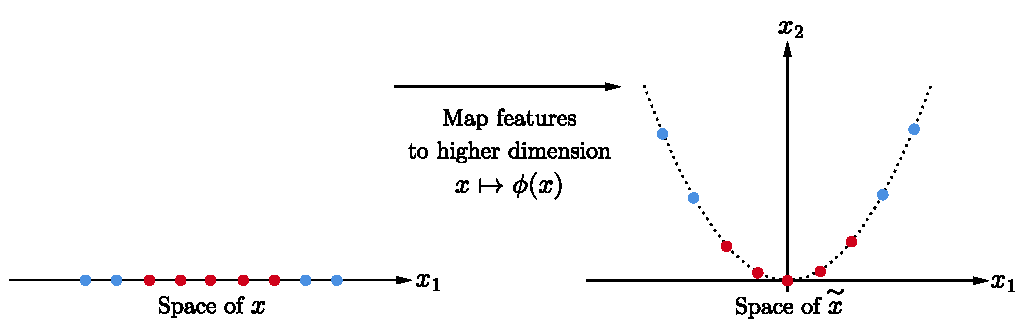
\includegraphics[width=0.8\textwidth]{figures/featuremapping.pdf}
	\caption{Principle of mapping features $x$ to a higher dimension with an appropriate mapping function $\phi(x)$, such that the features might become separable using a hyperplane in the new space.}
	\label{fig:featuremapping}
\end{figure} The same optimization framework is applicable as for basic SVMs; one just needs to replace every $x^{(i)}$ with $\phi(x^{(i)})$. Also, the prediction on a new sample $x^{(i)}$ needs to be then made with 
\begin{equation}
	y^{(k)} = \begin{cases}
		+1, &\quad w^{*\top}\phi\left(x^{(k)}\right) + b^* > 0 \\
		-1, &\quad w^{*\top}\phi\left(x^{(k)}\right) + b^* < 0
	\end{cases}.
\end{equation}
}

\Que{What is a kernel (matrix) in the context of SVMs and why is it useful?}
\Ans{
A key quantity occurring in the equations of SVMs is the inner product $(x^{(i)})^\top x^{(j)}$ for $i,j=1,\dots,m$ for a dataset containing $m$ samples $(x^{(i)},y^{(i)})$. Now, if one uses feature mapping, this inner product becomes \begin{equation}
	(x^{(i)})^\top x^{(j)} \mapsto \phi(x^{(i)})^\top \phi(x^{(j)}) \doteq K(x^{(i)},x^{(j)}).
\end{equation} Because this is a re-occurring expression in the SVM equations, one defines this quantity as the so-called kernel $K(x,z)$. One can use and experiment with different kernels when using SVMs to try to separate non-linearly separable datasets. Oftentimes, it is very useful to calculate the kernel directly, instead of first calculating $\phi(x)$ and $\phi(z)$ and then taking the inner product $\phi(x)^\top \phi(z)$. 

Hereby, the Mercer theorem is very useful: If a kernel $K: \mathbb{R}^n \times \mathbb{R}^n \rightarrow \mathbb{R}$ written as kernel matrix for input vectors $\{x^{(1)},\dots,x^{(m)}\}$ with $m < \infty$ is positive semi-definite, then one can write the kernel in the form $K(x^{(i)},x^{(j)}) = \phi(x^{(i)})^\top \phi(x^{(j)})$. Thus, if the Mercer theorem is fulfilled for some chosen kernel, then one has found an ``allowed'' feature mapping and potentially a way to calculate the inner product of the feature mappings much more efficiently than explicitly defining and calculating the feature mappings and then performing the inner product. 
}

\Que{How can the fundamental optimization problem for support vector machines be solved?}
\Ans{
Given a dataset $(x^{(i)},y^{(i)})$ of feature vectors $x \in \mathbb{R}^n$ and labels $y\in\{-1,+1\}$ with $i=1,\dots,m$, the central problem to solve in SVM algorithms is \begin{equation}
	\alpha^* = \arg\max_{\substack{\alpha: \text{Constraints}}}\underbrace{\left[\sum_{i=1}^{m}\alpha_i - \frac{1}{2}\sum_{i,j=1}^{m}\alpha_i\alpha_jy^{(i)}y^{(j)}(x^{(i)})^\top x^{(j)}\right]}_{\doteq\, W(\alpha)}.
\end{equation} Here, the constraints can e.g. be $\alpha_i \geq 0$ for all $i \in \{1,\dots,m\}$. The so-called SMO (sequential minimal optimization) algorithm can be used to solve that minimization/maximization problem. 

The SMO algorithm works by means of sequentially fixing all but two quantities $\alpha_i$ and $\alpha_j$ of the function $W(\alpha)$ which is to be maximized. Fixing all parameters but $\alpha_i$ does not work because of the constraint $\sum_{j=1}^{m}y^{(j)}\alpha_j = 0$ which yields \begin{equation}
	\alpha_i y^{(i)} +  \underbrace{\sum_{j\neq i}\alpha_jy^{(j)}}_{\doteq \gamma} = 0 \quad \Leftrightarrow \quad \alpha_i = -\gamma
\end{equation} and hence leaves no room for optimization. So all but two parameters $\alpha_i$ and $\alpha_j$ are fixed. Imposing the constraint $\sum_{l}\alpha_ly^{(l)} = 0$ yields \begin{equation}\label{eq:svmalphai}
\alpha_iy^{(i)} + \alpha_jy^{(j)} + \sum_{k\neq i,j}\alpha_ky^{(k)} = 0 \quad \Leftrightarrow \quad \alpha_i = -\alpha_jy^{(i)}y^{(j)} - y^{(j)}\sum_{k\neq i,j}\alpha_k y^{(k)},
\end{equation} where the parameters $\alpha_i$ and $\alpha_j$ are constrained to a box $[0,C]\times [0,C]$ by the condition $0 \leq \alpha_i \leq C$ for all $i = 1,\dots,m$, as \cref{fig:posslines} shows.
\begin{figure}[h]
	\centering
	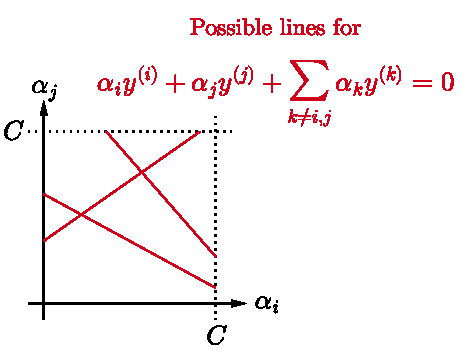
\includegraphics[width=0.4\textwidth]{figures/posslines.pdf}
	\caption{Possible values for the parameters $\alpha_i$ and $\alpha_j$ subject to the constraint $0 \leq \alpha_i \leq C$ for all $i=1,\dots,m$.}
	\label{fig:posslines}
\end{figure}
Now, one can substitute $\alpha_i$ in $W(\alpha_1,\dots, \alpha_i,\alpha_j,\dots,\alpha_m)$ with the above expression, which yields a function $W(\alpha_j)$ of only one variable $\alpha_j$, because all other parameters are fixed. This means, that one now finds $\alpha_j^*$ by means of \begin{equation}
\alpha_j^* = \arg\max_{\alpha_j} \left[W(\alpha_j)\right]
\end{equation} using for example a gradient ascent (or descent) method. Then, one can go about calculating $\alpha_j^*$ using \cref{eq:svmalphai}. Thus, the optimization in two parameters has been carried out. The SMO algorithm then iterates pair-wise through all other parameters, leading to the optimal solution $\alpha^*$.
}

\subsection{Decision trees} % Lecture 7/8
\Que{What is a decision tree and what is the principle of the decision tree method?}
\Ans{A decision tree is a very intuitive and useful approach for classification tasks. Consider a dataset $\{(x^{(i)},y^{(i)})\}_{i=1,\dots,m}$ of pairs of feature vectors $x \in \mathbb{R}^n$ and labels $y\in \{1,\dots,K\}$. A decision tree works by the principle of concatenating binary decisions to partition a parent partition $R_p$ into two child partitions $R_1$ and $R_2$. The goal is to finally have the samples belonging to each class separated in separate partitions.
	
Visually, decision trees can be explained as seen in \cref{fig:decisiontrees}.
\begin{figure}[h]
	\centering
	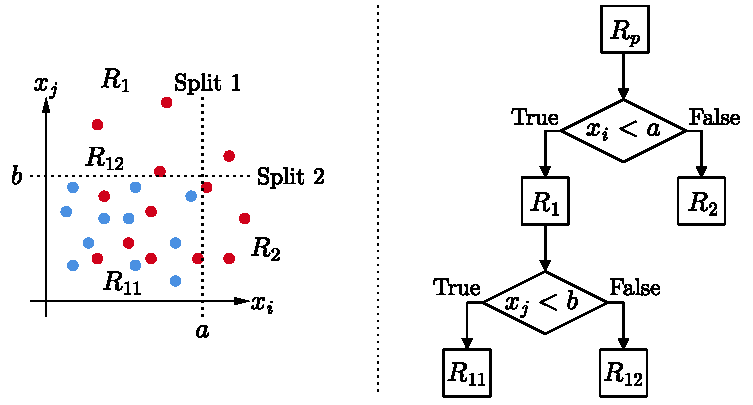
\includegraphics[width=0.6\textwidth]{figures/decisiontrees.pdf}
	\caption{Left panel: Decision tree working principle shown in a plane for $y \in \{1,2\}$ and features $x_i$ and $x_j$. Right panel: The same situation as seen in the left panel shown as decision tree.}
	\label{fig:decisiontrees}
\end{figure} Given a parent region $R_p$ consisting of samples $x$ of feature vectors, the child regions $R_1$ and $R_2$ given some threshold value $t$ applied to feature $x_j$ are calculated by \begin{align}\begin{aligned}
R_1 &= \{x|x_j < t, x \in R_p\},\\
R_2 &= \{x|x_j \geq t, x \in R_p\}.
\end{aligned}\end{align} Regarding the right panel of \cref{fig:decisiontrees}, every instance where a decision is made is called a leaf node (rhomboid structure). The depth of a decision tree is furthermore given by the maximal number of concatenated decisions (maximal number of concatenated rhomboid structures). Finally, we understand the cardinality of a certain leaf (square box) as leaf size.

In order to choose the splits, one requires a loss function $L(R)$, where $R$ is a region. This loss can generally be understood as the proportion of misclassified samples in $R$. Therefore, making a split one would like to decrease the proportion of misclassified samples in the splits $R_1$ and $R_2$ compared to a parent region $R_p$. One can define the quantity $D(R_p,R_1,R_2)$ denoting the decrease in terms of loss going from a parent region $R_p$ to two child regions $R_1$ and $R_2$ as \begin{equation}
	D(R_p, R_1, R_2) = L(R_p) - \frac{|R_1|L(R_1)+|R_2|L(R_2)}{|R_1|+|R_2|}.
\end{equation}
As a loss function, the cross-entropy loss \begin{equation}
	L_{ce}(R) = -\sum_c p_c(R)\log_2\left[p_c(R)\right],
\end{equation} is used, where $p_c(R)$ is the proportion of $c$-classified samples in $R$, namely \begin{equation}
p_c(R) = \frac{\text{Number of samples belonging to class $c$ in $R$}}{\text{Number of samples in $R$}}.
\end{equation} Using $L_{ce}(R)$ as a loss function ensures, that one always has a decrease $D(R_p, R_1, R_2)$ by splitting a parent region into two child regions.

There are three common stopping criteria for training a decision tree:
\begin{enumerate}
	\item Minimum leaf size: Do not split a region $R$ anymore, if its cardinality falls below a threshold $t$.
	\item Maximum depth: Do not split a region $R$ anymore, if a threshold $t$ of decisions have already been made in succession to reach $R$.
	\item Maximum number of nodes: Do not split a region $R$ anymore, if a maximum threshold $t$ of decisions have been made.
\end{enumerate}

Now, if a decision tree has been trained, there are a finite number of leafs $R_i$, $i=1,\dots,q$ and leaf nodes in the tree. The decision tree may be pictures as a function \begin{equation}
	f(x) = \begin{cases}
		1, &\quad x \in R_1 \\
		\vdots &\quad \vdots \\
		q, &\quad x \in R_q
	\end{cases}
\end{equation} Given a new sample $x^{(l)}$, one feeds that sample to the decision tree and checks, in which leaf $R_i$ it would end up; for example $f(x^{(l)}) = j$ for $j \in \{1,\dots,q\}$. Finally, one calculates $p_c(R_j)$ on the training data for all classes present in $R_j$, which will yield probabilities of the sample $x^{(l)}$ belonging to any of the classes $c$ in $R_j$. The sample $x^{(l)}$ is then classified as belonging to the class of highest probability in $R_j$.
}

\Que{What common two types of loss functions are there? What are the issues?}
\Ans{
The two common types of classification losses for training decision trees are the misclassification loss and the cross-entropy loss. In practice however, only the cross-entropy loss is used, because the misclassification loss has the issue, that there is no guarantee that it decreases when making splits.

The misclassification loss is defined as \begin{equation}
	L_{mc}(R) = 1-\max_c[p_c(R)],
\end{equation} whereas the cross-entropy loss is given by \begin{equation}
L_{ce}(R) = -\sum_c p_c(R)\log_2[p_c(R)].
\end{equation} Both loss functions are visualized in \cref{fig:dt_loss}.
\begin{figure}[h]
	\centering
	\begin{subfigure}{0.49\textwidth}
		\centering
		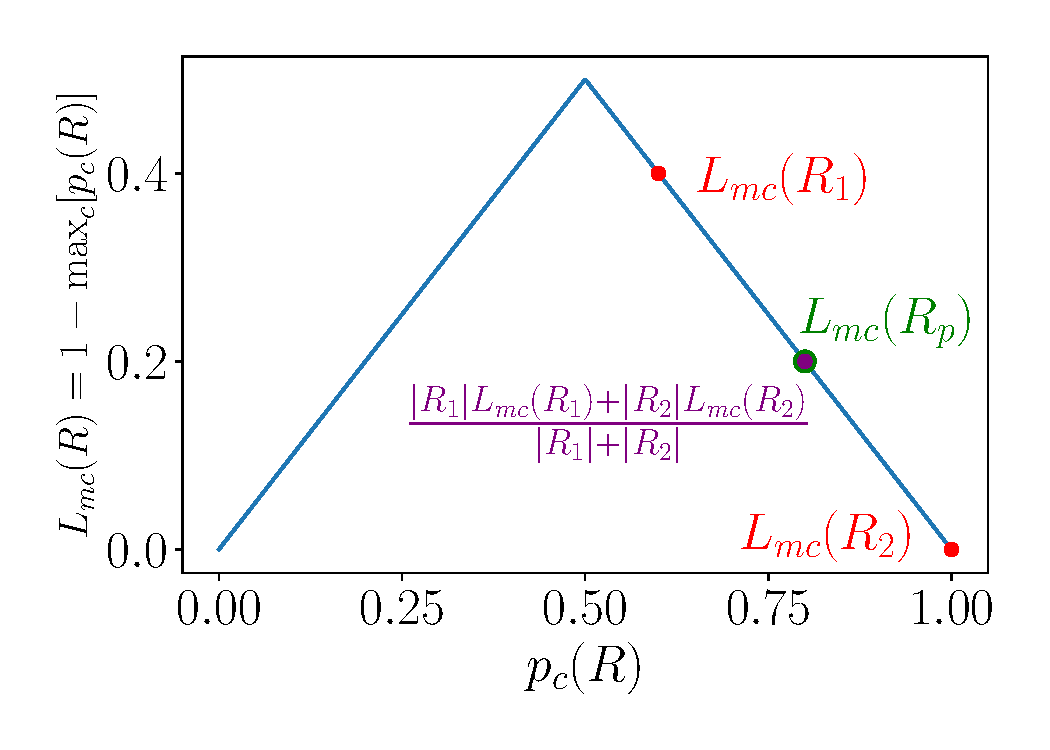
\includegraphics[width=\textwidth]{figures/dt_misclassification_loss.pdf}
		\caption{Misclassification loss for binary classification.}
		\label{fig:dt_misclassification_loss}
	\end{subfigure}
	\begin{subfigure}{0.49\textwidth}
		\centering
		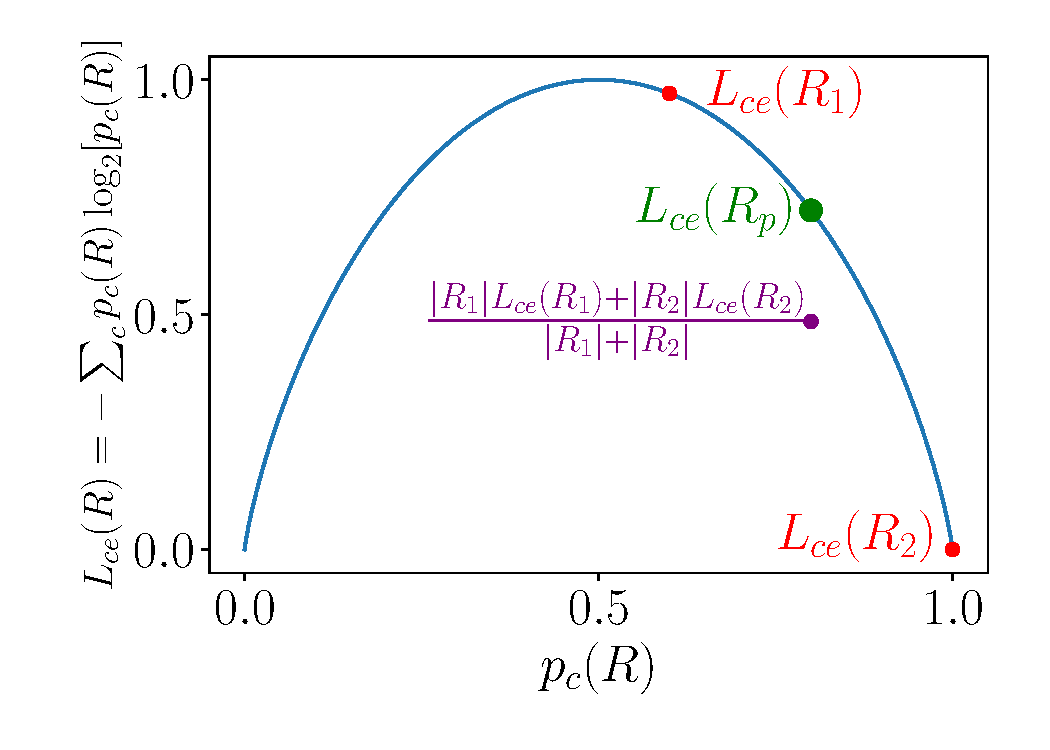
\includegraphics[width=\textwidth]{figures/dt_crossentropy_loss.pdf}
		\caption{Cross-entropy loss for binary classification.}
		\label{fig:dt_crossentropy_loss}
	\end{subfigure}
	\caption{Loss functions for training of decision trees. The figure was produced by assuming $R_p = \{400+, 100-\}$, $R_1 = \{150+,100-\}$ and $R_2 = \{250+, 0-\}$.}
	\label{fig:dt_loss}
\end{figure} As one can see from the figure, only for the cross-entropy loss, the decrease $D(R_p, R_1, R_2)$ in loss going from the parent $R_p$ to the children $R_1$ and $R_2$ is guaranteed to decrease.
}


\Que{What are the main advantages and disadvantages of the decision tree method?}
\Ans{
The advantages of decision trees are the following:
\begin{enumerate}
	\item[(A1)] Decision trees are easy to explain and interpretable.
	\item[(A2)] Decision trees support categorical variables (features); one does not have to first convert categorical variables to numbers.
	\item[(A3)] Decision trees are fast.
	\item[(A4)] Decision trees can capture non-linear patterns.
\end{enumerate}
The drawbacks of decision trees are the following:
\begin{enumerate}
	\item[(D1)] Decision trees lead to a high variance in predictions; this is mainly due to the fact that decision trees tend to overfit, as they continue to split regions until each leaf is ideally pure. This leads to capture of just nose, instead of capturing the general pattern behind the data. Therefore, also predictions will vary wildly; hence they have large variance.
	\item[(D2)] Decision trees cannot easily capture additive structure; that is, for example perform a split according to a linear function between two features. Many splits in a staircase-like manner are necessary to do that.
\end{enumerate}
}

\subsection{Ensembling methods} % Lecture 7/8
\Que{What is the general idea of ensembling methods?}
\Ans{
Consider a number of random variables $x_1,\dots,x_n$ with associated variances $\sigma_{x_i}^2\doteq \mathbb{V}(x_i)$ for $i=1,\dots,n$. Now, if each random variable $x_i$ is understood a the prediction of the $i$'th model, it is reasonable to compute an average prediction $\bar{x}$ as \begin{equation}
	\bar{x} = \frac{1}{n}\sum_{i=1}^{n}x_i.
\end{equation} It is now interesting to calculate the variance $\mathbb{V}(\bar{x})$ on the average prediction $\bar{x}$. Doing this, we obtain
\begin{align}
	\begin{aligned}
		\sigma_{\bar{x}}^2 &\doteq \mathbb{V}(\bar{x}) = \mathbb{V}\left(\frac{1}{n}\sum_{i=1}^n x_i\right) = \mathbb{E}\left[\left(\frac{1}{n}\sum_{i=1}^{n}x_i - \mathbb{E}\left[\frac{1}{n}\sum_{i=1}^n x_i\right]\right)^2\right] \\
		&=\mathbb{E}\left[\left(\frac{1}{n}\sum_{i=1}^{n}x_i - \frac{1}{n}\sum_{i=1}^n \mathbb{E} [x_i]\right)^2\right] = \mathbb{E}\left[\frac{1}{n^2}\left(\sum_{i=1}^{n}\left(x_i-\mathbb{E}[x_i]\right)\right)^2\right] \\
		&= \frac{1}{n^2}\mathbb{E}\left[\sum_{i=1}^{n}(x_i-\mathbb{E}[x_i])\sum_{j=1}^n(x_j-\mathbb{E})[x_j])\right] = \frac{1}{n^2}\mathbb{E}\left[\sum_{i,j=1}^n(x_i-\mathbb{E}[x_i])(x_j-\mathbb{E}[x_j])\right] \\
		&= \frac{1}{n^2}\mathbb{E}\left[\sum_{i=1}^{n}(x_i-\mathbb{E}[x_i])^2 + 2\sum_{1\leq i < j \leq n}(x_i-\mathbb{E}[x_i])(x_j-\mathbb{E}[x_j])\right] \\
		&= \frac{1}{n^2}\left(\sum_{i=1}^{n}\mathbb{E}\left[(x_i-\mathbb{E}[x_i])^2\right] + 2\sum_{1\leq i < j \leq n}\mathbb{E}\left[(x_i-\mathbb{E}[x_i])(x_j-\mathbb{E}[x_j])\right]\right) \\
		&= \frac{1}{n^2}\left(\sum_{i=1}^{n}\mathbb{V}(x_i)+ 2\sum_{1\leq i < j \leq n}\mathbb{K}(x_i,x_j)\right) = \frac{1}{n^2}\sum_{i=1}^{n}\sigma_{x_i}^2 + \frac{2}{n^2}\sum_{1\leq i < j \leq n} \rho(x_i,x_j)\sigma_{x_i}\sigma_{x_j},
	\end{aligned} 
\end{align} where $\rho(x_i,x_j)$ is the correlation coefficient defined by \begin{equation}
\rho(x_i,x_j) = \frac{\mathbb{K}(x_i,x_j)}{\sqrt{\mathbb{V}(x_i)\mathbb{V}(x_j)}},
\end{equation} which is evidently zero, if the covariance is zero. For perfect correlation or anticorrelation, the correlation coefficient is either $+1$ or $-1$, so $\rho(x_i,x_j) \in [-1,1]$.

Consider the case, where the random variables are identically distributed with correlation coefficient $\rho$, i.e. $\sigma_{x_i} = \sigma$ for all $i=1,\dots,n$. Then, the variance $\sigma_{\bar{x}}$ on the mean $\bar{x}$ is given by \begin{align}\begin{aligned}
	\sigma_{\bar{x}}^2 &=\frac{1}{n^2}\sum_{i,j=1}^{n}\mathbb{E}\left[(x_i-\mathbb{E}[x_i])(x_j-\mathbb{E}[x_j])\right] = \frac{1}{n^2}\sum_{i,j=1}^{n}\mathbb{K}(x_i,x_j) \\ &= \frac{1}{n^2}\left(\sum_{i=1}^{n}\mathbb{V}(x_i)+\sum_{\substack{i,j=1 \\ i\neq j}}^{n}\mathbb{K}(x_i,x_j)\right) = \frac{n\sigma^2}{n^2}+ \frac{1}{n^2}\sum_{\substack{i,j=1 \\ i\neq j}}^{n}\rho \sqrt{\mathbb{V}(x_i)\mathbb{V}(x_j)} \\ &= \frac{n\sigma^2}{n^2} + \frac{n(n-1)}{n^2}\rho\sigma^2 = \rho\sigma^2 + \frac{\sigma^2(1-\rho)}{n}.
\end{aligned}\end{align} And if it is the case that the random variables are furthermore identically and independently distributed, we have $\rho=0$ because of the correlations being zero, meaning that \begin{equation}
\sigma_{\bar{x}}^2 = \frac{\sigma^2}{n}.
\end{equation}

The general idea behind ensembling methods is therefore to find several models to make a prediction on the same sample; these predictions can be denoted by the random variables $x_1,\dots,x_n$. Depending on the correlation $\rho(x_i,x_j)=\frac{\mathbb{K}(x_i,x_j)}{\sqrt{\mathbb{V}(x_i)\mathbb{V}(x_j)}}$ between the models and the variances $\mathbb{V}(x_i)$, the resulting average prediction given by $\bar{x} = \frac{1}{n}\sum_{i=1}^nx_i$ will have a lower variance than the lowest of all predictions; it can however also be larger, this entirely depends on the incoming variances and correlations. In general therefore, in order to achieve a better performance of the ensembled method in comparison to individual methods, one needs to decrease correlation (decrease $\rho$) between models aswell as provide as many models as possible (increase $n$).
}

\Que{What methods are there to decorrelate methods in an ensemble of methods? What is decorrelation for?}
\Ans{
The term decorrelation refers to a strategy in ensembling methods to lower the resulting variance on predictions of the ensembled method. Given the equation \begin{equation}
	\sigma_{\bar{x}} = \rho\sigma^2 + \frac{\sigma^2(1-\rho)}{n}, \quad \bar{x} = \frac{1}{n}\sum_{i=1}^n x_i,
\end{equation} where we have assumed that the $x_i$ are identically distributed, we can either increase the amount $n$ of models in the ensemble or decrease the correlations $\rho$ to achieve precisely that; decorrelation refers to the latter. There are four prominent ways to do decorrelation:
\begin{enumerate}
	\item Using different algorithms.
	\item Using different training sets.
	\item Bagging.
	\item Boosting.
\end{enumerate}
}

\Que{How does bagging work?}
\Ans{
Bagging stands for bootstrap aggregation and is a technique used in ensembling methods for variance reduction. Assume, one has a dataset $S= \{(x^{(i)},y^{(i)})\}{i=1,\dots,m}$ of samples, where $x\in \mathbb{R}^n$ are feature vectors and $y$ class labels. With the bagging method, one aggregates low-bias, high-variance models to aim for variance reduction.

One samples several subsets $S_i \subseteq S$ and trains models $h_{i,\theta_i}$ for $i =1,\dots,M$ on those sets. Typically, these trained models will be quite accurate (low-bias), but have a high variance. These models are then aggregated by means of defining a new predictor as \begin{equation}
	h_\theta(x) = \frac{1}{M}\sum_{i=1}^M h_{i,\theta_i}(x).
\end{equation} This method is called bagging.
}

\Que{How does boosting work?}
\Ans{
Boosting is a technique used in ensembling methods for bias reduction. Assume, one has a dataset $S= \{(x^{(i)},y^{(i)})\}{i=1,\dots,m}$ of samples, where $x\in \mathbb{R}^n$ are feature vectors and $y$ class labels. With the boosting method, one aggregates high-bias, low-variance models to aim for bias reduction.

Towards this aim, one successively aggregates and trains $M$ high-bias models (e.g. linear regression or single-step decision trees) $h_{i,\theta_i}$ on the data $S$ as \begin{equation}
	G_k(x) = G_{k-1}(x) + h_{k,\theta_k}(x), \quad G_1(x) = h_{1,\theta_1}(x)
\end{equation} for $k \in \mathbb{M}$. Each subsequent model $G_{i}(x)$ gives particular weight to the misclassifications of the previous model $G_{i-1}(x)$. The final model is then given by \begin{equation}
h_{\theta}(x) = \frac{1}{M}G_M(x).
\end{equation} This predictor will have an increased accuracy due to bias reduction.
}

\Que{How are methods actually combined/ensembled to make a prediction?}
\Ans{
Say one has a supervised learning problems, where $x$ are feature vectors and $y$ are labels. Then we assume, that we have $m$ different models given by hypothesis functions $h_{1,\theta_1}(x), \dots,h_{m,\theta_m}(x)$ with uncertainties $\sigma_1,\dots,\sigma_m$ and correlations $\rho_{ij}$ associated with them. In order to make a prediction on a sample $x^{(k)}$ using the ensemble of methods, one simply calculates \begin{equation}
	y^{(k)} = \frac{1}{m}\sum_{i=1}^mh_{i,\theta_i}(x^{(k)}),
\end{equation} where the resulting uncertainty $\sigma_y$ on the prediction is given by \begin{equation}
\sigma_{y}^2 = \frac{1}{m^2}\sum_{i=1}^m\sigma_i^2 + \frac{2}{m^2}\sum_{1\leq i < j \leq m}\rho_{ij}\sigma_i\sigma_j.
\end{equation}
}

\subsection{Regularization and model selection}
\Que{What is regularization?}
\Ans{
Regularization describes a family of approaches that ensure, that a trained model generalizes well. That is to say, regularization aims for the goal of good performance of a trained model on unseen data. 

Consider for example, that one has a set $M = \{M_1,\dots,M_n\}$ of $n$ models trained on a dataset $S$. Assume, that $M_k$ is a $k$-th order polynomial model. It is known, that a higher order polynomial will better fit the training data $S$. However, one will also fit the uncertainty present in the training data $S$, which will lead to bad performance on new, unseen data. One calls this overfitting; and regularization is the means to prevent a model from overfitting during training. % Lecture 8
}

\Que{What are train, validation and test splits for?}
\Ans{
Given some model $M$ and a training dataset $S = \{(x^{(i)}, y^{(i)})\}_{i=1,\dots,m}$, one usually divides the data into training and testing data as \begin{equation}
	S_{test} \subset S, \qquad S_{train} \subset S, \qquad S_{test} \cap S_{train} = \emptyset, \qquad S_{test} \cup S_{train} = S.
\end{equation} The training set $S_{train}$ is only used to train the model $M$, while the test set $S_{test}$ is solely used to test the model after final training. There however is also such a thing as the validation set. The validation set is used to determine the optimal hyperparameters for the model $M$, such as the polynomial degree for a polynomial regression model. Oftentimes, the validation set is chosen as a subset of the training dataset (e.g. via the cross validation technique). The reason why the test dataset is not used for hyperparameter setting is that one would use information gained by the test dataset to ``improve'' the model; but that could lead to overfitting and less performance on unseen data; the test data would thus become some sort of training data.
 % Lecture 8
}

\Que{How does hold-out cross validation (simple cross validation) work and what are its disadvantages?}
\Ans{
Consider an available dataset $S$ on which we would like to train models $M_1,\dots,M_d$ of the same family, but with different hyperparameters. In order to find the optimal hyperparameters, one needs to train the models $M_i$ on a training dataset, evaluate their performance on a validation set and finally give the test performance for the model with least error on the validation set.

Now, so-called hold-out cross validation, also known as simple cross validation, is the simplest validation technique there is; it works as follows:
\begin{enumerate}
	\item Randomly split $S$ into $S_{train}$ and $S_{test}$ to, say 70 to 30 percent. Then, randomly split $S_{train}$ into a set $S_{tr}$ solely used for training, and a validation set $S_{val}$ only used for validation. Again, a typical split is 70 to 30 percent.
	\item Train each model $M_i$ on $S_{tr}$ to get a hypothesis function $h_{\theta_i}$; calculate the error $\varepsilon_{val}(h_{\theta_i})$ of each hypothesis function on the validation set $S_{val}$.
	\item Select the model $M_k$ with the smallest error $\varepsilon_{val}(h_{\theta_k})$ as the best model and output its performance on the test set $S_{test}$ as a final answer.
\end{enumerate}

The disadvantage of simple cross validation is that one needs to have a lot of data available, because one uses a large part of the original dataset $S$ just to validate the models and thus in a sense ``wastes'' data. However, compared to other approaches, simple cross validation is fast to use. Therefore, simple cross validation it is a good choice for situations in which data is abundant and/or one has models $M_i$ demanding a lot of computational resources (i.e. models with many model parameter).
}

\Que{How does k-fold cross validation work and what are its disadvantages?}
\Ans{
Consider an available dataset $S$ on which we would like to train models $M_1,\dots,M_d$ of the same family, but with different hyperparameters. In order to find the optimal hyperparameters, one needs to train the models $M_i$ on a training dataset, evaluate their performance on a validation set and finally give the test performance for the model with least error on the validation set.

Now, so-called k-fold cross validation is an advanced technique to do validation; it works as follows:
\begin{enumerate}
	\item Randomly split $S$ into $S_{train}$ and $S_{test}$ to, say 70 to 30 percent. Then, randomly split $S_{train}$ with cardinality $|S_{train}| = m$ into $k$ disjoint subsets $S_1,\dots,S_k$, each with cardinality $m/k$.
	\item For each model $M_i$, evaluate as follows:
	\begin{itemize}
		\item[] For $j = 1,\dots,k$ do the following:
		\begin{itemize}
			\item[] Train the model $M_i$ on $S_{train}\backslash S_j$ to get hypothesis function $h_{\theta_{ij}}$.
			\item[] Evaluate the error $\varepsilon_{ij}(h_{\theta_{ij})}$ of the hypothesis function $h_{\theta_{ij}}$ on the left-out set $S_j$ (validate $h_{\theta_{ij}}$ on $S_j$).
		\end{itemize}
		\item[] Calculate generalization error $\varepsilon_{i} = \frac{1}{k}\sum_{j=1}^{k}\varepsilon_{ij}(h_{\theta_{ij}})$.
	\end{itemize}
	\item Select the model $M_i$ with the smallest error $\varepsilon_i$ as the best model, train it on the entire set $S_{train}$ and output its performance on the test set $S_{test}$ as a final answer.
\end{enumerate}

The disadvantage of k-fold cross validation is that one needs to train a model $M_i$ for $k$ times. Especially for complex models with many parameters, this is expensive in terms of computational resources, but however ``wastes'' as little data as possible. Thus, k-fold cross validation is an ideal choice if the available dataset $S$ is sparse and/or if the models $M_i$ do not require heavy computational resources (i.e. models with a small amount of parameters). % Lecture 8
}

\Que{What is feature selection, when is it useful and how does it work?}
\Ans{
Consider a dataset $\{(x^{(i)},y^{(i)})\}_{i=1,\dots,m}$ of feature vectors $x\in\mathbb{R}^n$ and labels $y$. It may very well be the case, that not all features are very relevant to make a prediction about the label. For example, if a feature $x_i$ would be completely irrelevant to a prediction on $y$, then $p(y|x_i) = p(y)p(x_i)$ would hold, i.e. that $p(y)$ and $p(x_i)$ are independent. However, in general there must be some correlation of $x$ and $y$ such that one can establish a model $h_\theta(x) = y$.

Feature selection helps to find an appropriate subset of features to consider when building a model. Only considering the relevant features for model fitting, one reduces overfitting; thus, the technique of feature selection is a regularization technique. There are two prominent ways to select features, the so-called forward search and backward search.

\paragraph*{Forward search algorithm}
\begin{enumerate}
	\item Initialize the feature set $F$ as $F= \emptyset$.
	\item Repeat the following tasks:
	\begin{itemize}
		\item[] For each feature $i = 1,\dots,n$ do the following:
		\begin{itemize}
			\item[] If $i \notin F$, let $F_i = F \cup \{i\}$. 
			\item[] Train model using only features in $F_i$, estimate generalization error $\varepsilon_i$ using cross validation.
		\end{itemize} 
		\item[] Set $F$ to be the feature subset $F_j$ with smallest generalization error $\varepsilon_j$, i.e. pick $j = \arg\min_i(\varepsilon_i)$ and set $F \leftarrow F \cup \{j\}$.
	\end{itemize}
	\item Select and output the best feature subset evaluated in the search procedure.
\end{enumerate}

\paragraph*{Backward search algorithm}
\begin{enumerate}
	\item Initialize the feature set $F$ as $F= \{1,\dots,n\}$.
	\item Repeat the following tasks:
	\begin{itemize}
		\item[] For each feature $i = 1,\dots,n$ do the following:
		\begin{itemize}
			\item[] If $i \in F$, let $F_i = F\backslash \{i\}$. 
			\item[] Train model using only features in $F_i$, estimate generalization error $\varepsilon_i$ using cross validation.
		\end{itemize} 
		\item[] Set $F$ to be the feature subset $F_j$ with smallest generalization error $\varepsilon_j$, i.e. pick $j = \arg\min_i(\varepsilon_i)$ and set $F \leftarrow F \backslash \{j\}$.
	\end{itemize}
	\item Select and output the best feature subset evaluated in the search procedure.
\end{enumerate} 

The forward search algorithm should be employed, if one is confident that less than half $< n/2$ of the features are relevant for label prediction, whereas backward search can be used, if it seems more likely that more than half $>n/2$ of the features correlate to the labels.% Lecture 9
}

\Que{What is mutual information and why is it used as a score function? What happens, if the two input quantities to mutual information are independent?}
\Ans{
Mutual information is another way to prevent overfitting by selecting and using only those features for training, which seem relevant for label prediction. That is to say, mutual information can help at feature selection. In order to assess, if a feature $x_i$ of a feature vector $x \in \mathbb{R}^n$ is relevant te predict the label $y$, one can use mutual information defined as \begin{equation}
	\text{MI}(x,y) = \sum_{x}\sum_{y} p(x,y)\ln\left(\frac{p(x,y)}{p(x)p(y)}\right) \overset{\text{$x,y$ are cont.}}{=} \int_\mathbb{R}\int_\mathbb{R}p(x,y)\ln\left(\frac{p(x,y)}{p(x)p(y)}\right)\,\mathrm{d}x\,\mathrm{d}y.
\end{equation} By definition, mutual information is non-negative. Thus, for example, if some feature is completely irrelevant to predict $y$, then $p(x_i,y) = p(x_i)p(y)$ and thus \begin{equation}
\text{MI}(x_i,y) = \sum_{x}\sum_{y} p(x_i)p(y)\ln\left(\frac{p(x_i)p(y)}{p(x_i)p(y)}\right) = 0.
\end{equation} Thus, if another feature $x_j$ were correlated to $y$, then $\text{MI}(x_j,y) > 0$. 

Using mutual information and an appropriate threshold $t$, one can thus consider only those features $x_j$ for training the model, whose mutual information $\text{MI}(x_j,y)$ is above the threshold $t$.
}

\Que{What is the relation of mutual information to the Kullback-Leibler divergence?}
\Ans{
Consider a random variable $x\in \mathbb{R}^n$ and two distinct densities $p(x)$ and $q(x)$ on $x$.

The Kullback-Leibler divergence is a metric that quantifies the similarity of $p(x)$ to $q(x)$ and is accordingly defined as \begin{equation}
	\text{KL}(p(x),q(x)) \doteq \text{KL}(p||q) = \sum_{x}p(x)\ln\left[\frac{p(x)}{q(x)}\right] \overset{\text{$x$, $y$ are cont.}}{=} \int_{\mathbb{R}} p(x)\ln\left[\frac{p(x)}{q(x)}\right]\,\mathrm{d}x.
\end{equation} Consider now an additional random variable $y \in \mathbb{R}^k$ and a joint probability density $p(x,y)$. Then, one can see that the mutual information of $x$ and $y$ is the Kullback-Leibler divergence of the probability densities $p(x,y)$ and $p(x)p(y)$, namely \begin{equation}
\text{MI}(x,y) = \text{KL}(p(x,y)||p(x)p(y)).
\end{equation} Mutual information hence calculates a measure of similarity between the joint density $p(x,y)$ and the density product $p(x)p(y)$. If this similarity is large, the mutual information will be very low as the Kullback-Leibler divergence will be near zero. However, if the similarity is nearly not present, the Kullback-Leibler divergence will be very large.
}

\Que{How are Bayesian statistics used for regularization?}
\Ans{
Conceiving of the weights $\theta$ of a model not as being unknown and constant, but as being unknown and a random variable following the density $p(\theta)$, one can derive the optimal weights $\hat{\theta}$ as \begin{equation}
	\hat{\theta} = \arg\max_\theta\left(\prod_{i=1}^{m}p(y^{(i)}|x^{(i)},\theta)p(\theta)\right)
\end{equation} using Bayesian statistics. This technique is known as maximum a posteriori estimation. Compared to the maximum likelihood estimation technique, we have an added term $p(\theta)$ here, which takes care of regularization. Due to this term, the found weights using maximum a posteriori estimation will generally have a smaller norm than those of maximum likelihood estimation and are thus less sensitive to fluctuations in new data $x^{(k)}$, $y^{(k)}$; this means, that a model trained using maximum a posteriori estimation will generalize better than a maximum likelihood trained one.
}

\section{Unsupervised learning}
\Que{What is unsupervised learning? What is the goal of unsupervised learning?}
\Ans{
Suppose that one has a dataset $\{x^{(i)}\}_{i=1,\dots,m}$ of feature vector $x\in\mathbb{R}^n$ samples. Unsupervised learning is about learning the parameters $\theta$ of a model that models a probability density $p(x; \theta)$. % Lecture 9
}

\subsection{Clustering and k-means} % Lecture 9
\Que{How does the k-means algorithm work?}
\Ans{The k-means algorithm is an algorithm belonging to the group of unsupervised learning algorithms. That is to say, we have a training set $\{x^{(1)}, \dots, x^{(m)}\}$ of training samples without labels, where the feature vectors $x \in \mathbb{R}^n$. The k-means algorithm aims to cluster these samples into $k$ classes centered around mean values $\mu_1,\dots,\mu_k$ of those classes. Once trained, new samples $x^{(l)}$ are assigned the class label $c^{(l)}$ as \begin{equation}
		  c^{(l)}  = \arg\min_i\left(\|x^{(l)}-\mu_i\|\right).
	\end{equation}
The algorithm works as follows:
\begin{enumerate}
	\item Initialize cluster centroids $\mu_1,\dots,\mu_k \in \mathbb{R}^n$ randomly.
	\item Repeat until convergence:
	\begin{itemize}
		\item[(a)] For every $i \in \{1,\dots,m\}$ of training dataset indices set
		$$ c^{(i)} = \arg\min_j\left(\|x^{(i)}-\mu_j\|\right). $$ This corresponds to assigning each sample $x^{(i)}$ to the class $j$ for which the distance $\|x^{(i)}-\mu_j\|$ is minimal.
		\item[(b)] For each $j \in \{1,\dots,k\}$ of class indices set 
		$$ \mu_j = \frac{\sum_{i=1}^{m}\mathbb{I}(c^{(i)}=j)x^{(i)}}{\sum_{i=1}^{m}\mathbb{I}(c^{(i)}=j)}. $$ This corresponds to updating the mean values of elements $x^{(i)}$ in cluster $j$.
	\end{itemize}
\end{enumerate}

The k-means algorithm can be shown to converge in the sense that the distortion function given by \begin{equation}
	J(c,\mu) = \sum_{i=1}^{m}\|x^{(i)} - \mu_{c^{(i)}}\|^2
\end{equation} is minimized. The distortion function measures the sum of squared distances of samples $x^{(i)}$ from their respective class mean $\mu_{c^{(i)}}$.
}

\Que{How do Gaussian mixture models work?}
\Ans{Gaussian mixture models (GMMs) are a probabilistic approach for clustering and density estimation in unsupervised learning. Suppose we have a dataset $\{x^{(i)}\}_{i=1,\dots,m}$ where each $x^{(i)} \in \mathbb{R}^n$ is a feature vector. GMM assumes that the data is generated from a mixture of $k$ Gaussian distributions, where each data point belongs to one of $k$ clusters with certain probabilities.
	
	To define GMM, we introduce latent variables $z^{(i)} \in \{1, \dots, k\}$, which indicate the cluster assignment of $x^{(i)}$. The model specifies:  
	\begin{itemize}
		\item The latent variables $z^{(i)}$ follow a multinomial distribution, where $\phi = \{\phi_1, \dots, \phi_k\}$ are the mixing proportions (probabilities of choosing each cluster) with $\phi_j \geq 0$ and $\sum_{j=1}^k \phi_j = 1$. Hence, we have $p(z^{(i)}=j;\phi) = \phi_j$. 
		\item The probability $p(x^{(i)}| z^{(i)} = j;\mu,\Sigma)$ is chosen to follow a Gaussian distribution. Hence, we have $p(x^{(i)}| z^{(i)} = j;\mu,\Sigma) = \mathcal{N}(\mu_j, \Sigma_j)$, a Gaussian distribution with mean $\mu_j$ and covariance $\Sigma_j$.
	\end{itemize}
	
	The function to maximize is the likelihood of the data $\{x^{(i)}\}_{i=1,\dots,m}$. Given the model parameters $\phi, \mu$ and $\Sigma$, that is to maximize the function \begin{equation}
		f(\phi,\mu,\Sigma) = \sum_{i=1}^{m}p(x^{(i)};\phi,\mu,\Sigma)
	\end{equation} with respect to the model parameters $\phi$, $\mu$ and $\Sigma$. Using marginalization $p(x) = \int p(x|z)p(z)\,\mathrm{d}z$ for any random variables $x$ and $z$, furthermore leveraging te IID assumption aswell as taking the natural logarithm, the function to maximize $l(\phi,\mu,\Sigma)$ reads as \begin{equation}
	l(\phi,\mu,\Sigma) = \sum_{i=1}^m \ln \left( \sum_{j=1}^k p(x^{(i)} | z^{(i)} = j; \mu_j, \Sigma_j) p(z^{(i)} = j; \phi_j) \right).
	\end{equation} Maximizing $l(\phi,\mu,\Sigma)$ is equivalent to maximizing $f(\phi,\mu,\Sigma)$ from above. Now, since the latent variables $z^{(i)}$ (which are a ``simulation of labels $y^{(i)}$'') are unobserved, directly maximizing the likelihood to estimate the parameters $(\phi, \mu, \Sigma)$ is not tractable. If the $z^{(i)}$ were known as in the case of $y^{(i)}$ in a supervised learning problem, the function to maximize would read \begin{equation}
	\ell(\phi,\mu,\Sigma) = \sum_{i=1}^{m}\left(\ln\left[p(x^{(i)}|z^{(i)};\mu,\Sigma)\right] + \ln\left[p(z^{(i)};\phi)\right]\right),
	\end{equation} leading to a closed form solution of the maximization culminating in the model parameters given by \begin{align}
	\begin{aligned}
		\phi_j &= \frac{1}{m}\sum_{i=1}^{m}\mathbb{I}\{z^{(i)} = j\}, \\
		\mu_j &= \frac{\sum_{i=1}^{m}\mathbb{I}\{z^{(i)}=j\}x^{(i)}}{\sum_{i=1}^{m}\mathbb{I}\{z^{(i)} = j\}}, \\
		\Sigma_j &= \frac{\sum_{i=1}^{m}\mathbb{I}\{z^{(i)}=j\}(x^{(i)}-\mu_j)(x^{(i)}-\mu_j)^\top}{\sum_{i=1}^{m}\mathbb{I}\{z^{(i)}=j\}}.
	\end{aligned}
	\end{align}
	
	In expectation maximization however, this is not possible and there exists no closed-form solution to the maximization (minimization) problem. The expectation maximization (EM) algorithm consists therefore of an estimation (expectation, E) step and a maximization (M) step, which are repeated iteratively until convergence. It works as follows: 
	\begin{enumerate}
		\item \textbf{E-step}: Compute the posterior probabilities (soft assignments) of the latent variables by leveraging the Bayes theorem:  
		\[
		w^{(i)}_j = p(z^{(i)} = j | x^{(i)}; \phi, \mu, \Sigma) = \frac{p(x^{(i)} | z^{(i)} = j; \mu_j, \Sigma_j)p(z^{(i)} = j; \phi_j)}{\sum_{l=1}^k p(x^{(i)} | z^{(i)} = l; \mu_l, \Sigma_l)p(z^{(i)} = l; \phi_l)}.
		\] 
		\item \textbf{M-step}: Update the parameters using the soft assignments similar to using the indicator functions as in the supervised learning problem algorithms:  
		\[
		\phi_j = \frac{1}{m} \sum_{i=1}^m w^{(i)}_j, \quad \mu_j = \frac{\sum_{i=1}^m w^{(i)}_j x^{(i)}}{\sum_{i=1}^m w^{(i)}_j}, \quad \Sigma_j = \frac{\sum_{i=1}^m w^{(i)}_j (x^{(i)} - \mu_j)(x^{(i)} - \mu_j)^\top}{\sum_{i=1}^m w^{(i)}_j}.
		\]  
	\end{enumerate}
	
	This iterative process repeats until convergence, typically when the log-likelihood stops improving significantly. The EM algorithm guarantees that the log-likelihood increases with each iteration. GMMs can be seen as a soft version of the k-means algorithm, where the hard cluster assignments are replaced by probabilistic assignments.
}

\subsection{EM and factor analysis} % Lecture 10
\Que{What is Jensen's inequality (equality) and what is it used for?}
\Ans{
Jensen's inequality is a useful tool in the expectation maximization (EM) algorithm, as it gives a lower bound to a maximization problem. Let $f(x)$ be a function of a random variable. Then, \begin{equation}
	\mathbb{E}[f(x)] \geq f(\mathbb{E}[x]) \quad \text{if} \quad \text{$f(x)$ is convex}
\end{equation} holds, whereas \begin{equation}
\mathbb{E}[f(x)] \leq f(\mathbb{E}[x]) \quad \text{if} \quad \text{$f(x)$ is concave}.
\end{equation} Convexity and concavity of the function $f(x)$ are given by the second derivative, i.e. $f(x)$ is convex if $\nabla_x^2 f(x) > 0$, whereas $f(x)$ is called concave, if $\nabla_x^2 f(x) < 0$.

There is a special case of Jensen's inequality, where it becomes an equality. Namely if the random variable $x$ is a constant, then one has \begin{equation}
	\mathbb{E}[f(x)] = f(\mathbb{E}[x]) \quad \text{if} \quad \text{$x$ is a constant}.
\end{equation}
} 

\Que{What is the intuition behind expectation maximization?}
\Ans{
Suppose, one has a training set $\{x^{(1)},\dots, x^{(m)}\}$ of unlabelled feature vectors $x \in \mathbb{R}^n$. Expectation maximization introduces a latent variable $z^{(i)} \in \{1,\dots,k\}$ for each sample, where $k$ is the number of assumed clusters. What one wants to learn with any unsupervised learning algorithm is the density $p(x;\theta))$, where $\theta$ are the model parameters. Expectation maximization exploits marginalization of $p(x;\theta)$ as \begin{equation}
	p(x;\theta) = \sum_{z}p(x,z;\theta) = p(x|z;\theta)p(z;\theta),
\end{equation} where one can make assumptions for both $p(x|z;\theta)$ and $p(z;\theta)$. For example, in Gaussian mixture models - which is a special case of an expectation maximization algorithm - one uses a Gaussian density for $p(x|z;\theta)$.
}

\Que{How is an expectation maximization method built?}
\Ans{
Suppose, one has a training set $\{x^{(1)},\dots, x^{(m)}\}$ of unlabelled feature vectors $x \in \mathbb{R}^n$.

Now, let $Q_i(z)$ be a probability density over the latent variable $z$ for each sample $i \in \{1,\dots,m\}$. What one would like to maximize is the probability \begin{equation}
	p(x^{(1)},\dots,x^{(m)};\theta) \overset{\text{I.I.D.}}{=} \prod_{i=1}^{m}p(x^{(i)};\theta).
\end{equation} Maximizing this expression with respect to the model parameters $\theta$ is the same as maximizing the logarithm of the same expression, that is \begin{gather}\small\begin{gathered}
\hat{\theta} = \arg\max_\theta\left(\prod_{i=1}^{m}p(x^{(i)};\theta)\right) = \arg\max_\theta\left(\ln\left[\prod_{i=1}^{m}p(x^{(i)};\theta)\right]\right) = \arg\max_\theta\left(\sum_{i=1}^{m}\ln\left[p(x^{(i)};\theta)\right]\right).
\end{gathered}\end{gather} We can thus calculate \begin{align}
	\begin{aligned}
		\ell(\theta) \doteq  \sum_{i=1}^m \ln\left[p(x^{(i)};\theta)\right] &= \sum_{i=1}^{m}\ln\left[\sum_{j=1}^k p(x^{(i)},z^{(i)}=j; \theta)\right]\\
		&= \sum_{i=1}^{m}\ln\left[\sum_{j=1}^k Q_i(z^{(i)}=j) \frac{p(x^{(i)},z^{(i)}=j; \theta)}{Q_i(z^{(i)}=j)}\right] \\
		&\geq \sum_{i=1}^{m}\sum_{j=1}^{k}Q_i(z^{(i)}=j)\ln\left[\frac{p(x^{(i)},z^{(i)}=j;\theta)}{Q_i(z^{(i)}j)}\right].
	\end{aligned}
\end{align} In the last step, Jensen's inequality for the convex function of the natural logarithm was used, namely \begin{equation}
\ln\left(\mathbb{E}_{z^{(i)}\sim Q_i}\left[\frac{p(x^{(i)},z^{(i)}=j;\theta)}{Q_i(z^{(i)}=j)}\right] \right) \geq \mathbb{E}_{z^{(i)}\sim Q_i}\left[\ln\left(\frac{p(x^{(i)},z^{(i)}=j;\theta)}{Q_i(z^{(i)}=j)}\right)\right],
\end{equation} where
\begin{equation}
\mathbb{E}_{z^{(i)}\sim Q_i}\left[\frac{p(x^{(i)},z^{(i)}=j;\theta)}{Q_i(z^{(i)}=j)}\right] = \sum_{j=1}^k Q_i(z^{(i)}=j)\frac{p(x^{(i)},z^{(i)}=j;\theta)}{Q_i(z^{(i)}=j)}
\end{equation} by definition of the expectation value with respect to $z^{(i)}$ drawn from $Q_i(z^{(i)})$. Equality holds per the Jensen inequality, if the random variable of which the expectation value is taken is constant. In the present case, that is if $p(x^{(i)},z^{(i)}=j;\theta)/Q_i(z^{(i)}=j)$ is a constant with respect to $z^{(i)}$. In this case we can write \begin{equation}
Q_i(z^{(i)}=j) = c\cdot p(x^{(i)},z^{(i)}=j;\theta) = c\cdot p(z^{(i)}=j|x^{(i)};\theta)p(x^{(i)};\theta).
\end{equation} Because $Q_i(z^{(i)}=j)$ is a probability, $\sum_{j=1}^kQ_i(z^{(i)}=j) = 1$ must hold and hence \begin{equation}
c = \frac{1}{p(x^{(i)};\theta)} \quad \Rightarrow\quad Q_i(z^{(i)}=j) = p(z^{(i)}=j|x^{(i)};\theta).
\end{equation} The lower bound for $\ell(\theta)$ is thus given by \begin{equation}
\sum_{i=1}^{m}\sum_{j=1}^{k}p(x^{(i)},z^{(i)}=j;\theta)\ln\left( \frac{p(x^{(i)},z^{(i)}=j;\theta)}{p(z^{(i)}=j|x^{(i)};\theta)}\right).
\end{equation} It can be shown from this and Jensen's inequality, that $\ell(\theta^{t=1}) \geq \ell(\theta^t)$ for any steps $t \rightarrow t+1$. Thus, the expectation maximization (EM) algorithm can be stated as \begin{equation}
\theta^{t+1} = \arg\max_\theta\left(\sum_{i=1}^m\sum_{j=1}^k p(z^{(i)}=j|x^{(i)};\theta^t)\ln\left[\frac{p(x^{(i)}|z^{(i)}=j;\theta)p(z^{(i)}=j;\theta)}{p(z^{(i)}=j|x^{(i)};\theta^t)}\right]
\right),
\end{equation} where $p(x^{(i)}|z^{(i)}=j;\theta)$ and $p(z^{(i)}=j;\theta)$ are assumed to be simple probability densities, e.g. Gaussians.

One can also express the update scheme as an E-step and an M-step, which are to be repeated until convergence:
\begin{enumerate}
	\item \textbf{E-step}: For each $i=1,\dots,m$, compute \begin{equation}
		Q_i(z^{(i)}=j) \doteq p(z^{(i)}=j|x^{(i)};\theta^t)
	\end{equation} for the current $\theta^t$ and all $j=1,\dots,k$.
	\item \textbf{M-step}: Set the new $\theta^{t+1}$ as \begin{equation}
		\theta^{t+1} \doteq \arg\max_\theta\left(\sum_{i=1}^{m}\sum_{j=1}^{k}Q_i(z^{(i)}=j)\ln\left[\frac{p(x^{(i)}|z^{(i)}=j;\theta)p(z^{(i)}=j;\theta)}{Q_i(z^{(i)}=j)}\right]\right).
	\end{equation}
\end{enumerate}
}

\Que{What is the intuition and the rationale for the factor analysis method?}
\Ans{
	Consider some training set $\{x^{(1)},\dots, x^{(m)}\}$ of unlabelled feature vectors $x \in \mathbb{R}^n$. I one would like to apply an EM algorithm, say a Gaussian mixture model, one would need to calculate covariance matrices \begin{equation}
		\Sigma_j = \sum_{i=1}^{m}(x^{(i)}-\mu_j)(x^{(i)}-\mu_j)^\top.
	\end{equation} There is no problem in doing that. But if we have the case $m < n$ or even $m \ll n$, meaning that the number of dimensions for the feature vectors (greatly) exceeds the sample size, one cannot calculate the inverses $\Sigma_j^{(-1)}$ anymore, as the matrices $\Sigma_j$ cannot be full rank by construction. This is because one can only have $m$ linearly independent vectors $x^{(i)} \in \mathbb{R}^n$ for a dataset of size $m$, thus forming a basis of the subspace $\mathbb{R}^m \subset \mathbb{R}^n$. Hence $m<n$, it can never be that the covariance matrix therefore is full rank. This is what makes it necessary to define an EM algorithm that also works for the case $m < n$.
}

\Que{How is factor analysis method built?}
\Ans{Factor analysis is used, when the sample size $m$ for a dataset $\{x^{(1)},\dots,x^{(m)}\}$ is strictly smaller than the dimensionality of the feature vectors $x \in \mathbb{R}^n$, that is $m < n$.
	
	The goal of factor analysis is to model the data using fewer parameters while capturing the correlation structure between dimensions. This is achieved by assuming that the observed data $x \in \mathbb{R}^n$ is generated as a linear combination of a smaller set of latent variables $z \in \mathbb{R}^k$ with added noise. Specifically, the generative model for factor analysis is given by
	\begin{align}
		z &\sim \mathcal{N}(0, I), \\
		x|z &\sim \mathcal{N}(\mu + \Lambda z, \Psi),
	\end{align}
	where $\mu \in \mathbb{R}^n$ is the mean vector, $\Lambda \in \mathbb{R}^{n \times k}$ is the factor loading matrix, and $\Psi \in \mathbb{R}^{n \times n}$ is a diagonal covariance matrix representing the noise. Here, $k < n$ is chosen to be smaller than the dimensionality of the data to ensure dimensionality reduction.
	
	Equivalently, this model can be expressed as
	\begin{equation}
		x = \mu + \Lambda z + \epsilon,
	\end{equation}
	where $z \sim \mathcal{N}(0, I)$ and $\epsilon \sim \mathcal{N}(0, \Psi)$ are independent.
	
	The joint distribution of $z$ and $x$ can then be written as
	\begin{equation}
		\begin{bmatrix}
			z \\ x
		\end{bmatrix} \sim \mathcal{N}\left(
		\begin{bmatrix}
			0 \\ \mu
		\end{bmatrix},
		\begin{bmatrix}
			I & \Lambda^\top \\
			\Lambda & \Lambda \Lambda^\top + \Psi
		\end{bmatrix}
		\right).
	\end{equation}
	From this, the marginal distribution of $x$ is
	\begin{equation}
		x \sim \mathcal{N}(\mu, \Lambda \Lambda^\top + \Psi).
	\end{equation}
	
	To fit the model parameters $\mu$, $\Lambda$, and $\Psi$ using the training data, one maximizes the log-likelihood of the observed data. However, this maximization cannot be solved in closed form due to the marginalization over the latent variables $z$. Hence, the expectation maximization (EM) algorithm is used. The EM steps for factor analysis are as follows:
	\begin{enumerate}
		\item \textbf{E-step:} Compute the posterior distribution $p(z^{(i)}|x^{(i)}; \mu, \Lambda, \Psi)$ for each data point $i \in \{1, \dots, m\}$. Using the properties of Gaussian distributions, this is given by
		\begin{align}
			\mu_{z^{(i)}|x^{(i)}} &= \Lambda^\top (\Lambda \Lambda^\top + \Psi)^{-1}(x^{(i)} - \mu), \\
			\Sigma_{z^{(i)}|x^{(i)}} &= I - \Lambda^\top (\Lambda \Lambda^\top + \Psi)^{-1} \Lambda.
		\end{align}
		\item \textbf{M-step:} Update the model parameters $\mu$, $\Lambda$, and $\Psi$ to maximize the expected complete-data log-likelihood. The updates are given by
		\begin{align}
			\mu &= \frac{1}{m} \sum_{i=1}^m x^{(i)}, \\
			\Lambda &= \left( \sum_{i=1}^m (x^{(i)} - \mu) \mathbb{E}[z^{(i)}]^\top \right) \left( \sum_{i=1}^m \mathbb{E}[z^{(i)} z^{(i)\top}] \right)^{-1}, \\
			\Psi &= \frac{1}{m} \sum_{i=1}^m \left[ (x^{(i)} - \mu)(x^{(i)} - \mu)^\top - \Lambda \mathbb{E}[z^{(i)}](x^{(i)} - \mu)^\top \right].
		\end{align}
		In the above, $\mathbb{E}[z^{(i)}] = \mu_{z^{(i)}|x^{(i)}}$ and $\mathbb{E}[z^{(i)} z^{(i)\top}] = \mu_{z^{(i)}|x^{(i)}} \mu_{z^{(i)}|x^{(i)}}^\top + \Sigma_{z^{(i)}|x^{(i)}}$ are the posterior expectations computed in the E-step.
	\end{enumerate}
	
	The algorithm alternates between the E-step and M-step until convergence, iteratively refining the estimates of $\mu$, $\Lambda$, and $\Psi$ to maximize the likelihood of the data under the factor analysis model.}


\subsection{PCA and ICA} % Lecture 11
\Que{What is the strategy of principal component analysis?}
\Ans{
	Consider some dataset feature vector sample $x^{(i)}$ given as \begin{equation}
		x^{(i)} = \begin{pmatrix}
			x_1^{(i)} \\ \vdots \\ x_n^{(i)}.
		\end{pmatrix}
	\end{equation} It could now be, that some of the components of $x^{(i)}$ were somehow related as say $x_j = 2x_k$. In that case, only one - either $x_j$ or $x_k$ - is to be considered a relevant feature. The strategy of principal component analysis is to eliminate all such redundancy and is thus a useful tool to preprocess data.
}

\Que{How does the principal component analysis (PCA) work?}
\Ans{
	The principal component analysis (PCA) works by identifying the subspace in which the data approximately lies, while preserving as much variance as possible in the data. Given a dataset $\{x^{(1)}, \dots, x^{(m)}\}$ of $m$ feature vectors $x^{(i)} \in \mathbb{R}^n$, PCA seeks to find a lower-dimensional representation of the data that captures the maximum variance.
	
	Before applying PCA, the data is typically pre-processed:
	\begin{enumerate}
		\item Subtract the mean $\mu = \frac{1}{m} \sum_{i=1}^m x^{(i)}$ from each $x^{(i)}$ to ensure zero mean.
		\item Normalize each feature to have unit variance if the scales of the features differ significantly.
	\end{enumerate}
	
	The PCA algorithm then works as follows:
	\begin{enumerate}
		\item Compute the covariance matrix of the data: 
		\begin{equation}
			\Sigma = \frac{1}{m} \sum_{i=1}^m x^{(i)} (x^{(i)})^\top.
		\end{equation}
		\item Perform eigenvalue decomposition of $\Sigma$ to find its eigenvectors and eigenvalues.
		\item Select the top $k$ eigenvectors $\{u_1, \dots, u_k\}$ corresponding to the largest $k$ eigenvalues. These eigenvectors form the principal components of the data.
		\item Project each $x^{(i)}$ onto the $k$-dimensional subspace spanned by $\{u_1, \dots, u_k\}$ to obtain the lower-dimensional representation:
		\begin{equation}
			y^{(i)} = \begin{pmatrix}
				u_1^\top x^{(i)} \\
				\vdots \\
				u_k^\top x^{(i)}
			\end{pmatrix} \in \mathbb{R}^k.
		\end{equation}
	\end{enumerate}
	
	This representation $y^{(i)}$ retains the maximum variance in the original data while reducing its dimensionality. PCA can be used for dimensionality reduction, noise reduction, and data visualization.
	}

\Que{What is the strategy of independent component analysis?}
\Ans{
	The strategy of independent component analysis (ICA) is to decompose a set of observed mixed signals into a set of statistically independent source signals. ICA assumes that the observed data $x \in \mathbb{R}^n$ is a linear mixture of independent components $s \in \mathbb{R}^n$:
	\begin{equation}
		x = A s,
	\end{equation}
	where $A$ is an unknown mixing matrix. The goal of ICA is to estimate the unmixing matrix $W = A^{-1}$ such that the independent sources can be recovered as $s = Wx$.
	
	A key application of ICA is the "cocktail party problem," where overlapping sounds from multiple speakers are separated using recordings from multiple microphones. ICA exploits the statistical independence of the sources to achieve this separation.}

\Que{How does the independent component analysis (ICA) work?}
\Ans{
	Independent component analysis (ICA) works by leveraging the assumption of statistical independence between the sources to estimate the unmixing matrix $W$. The algorithm can be summarized as follows:
	\begin{enumerate}
		\item Assume that the sources $s_i$ are independent and non-Gaussian, and their joint density can be written as:
		\begin{equation}
			p(s) = \prod_{i=1}^n p_s(s_i),
		\end{equation}
		where $p_s(s_i)$ is the probability density of the $i$-th source.
		\item Model the observed data as $x = A s$, where $A$ is the unknown mixing matrix, and rewrite the density of $x$ as:
		\begin{equation}
			p(x) = \prod_{i=1}^n p_s\left(w_i^\top x\right) \det(W),
		\end{equation}
		where $W = A^{-1}$ is the unmixing matrix, and $w_i^\top$ is the $i$-th row of $W$. The matrix $W \in \mathbb{R}^{n \times n}$ can be written explicitly as:
		\begin{equation}
			W = \begin{pmatrix}
				w_1^\top \\
				w_2^\top \\
				\vdots \\
				w_n^\top
			\end{pmatrix},
		\end{equation}
		where $w_i \in \mathbb{R}^n$ for each $i$.
		\item Define a reasonable density function $p_s$ for the sources, such as the derivative of the sigmoid function $g(s) = \frac{1}{1 + e^{-s}}$ given by $f(s) = \frac{\mathrm{d}g(s)}{\mathrm{d}s} = g(s)(1-g(s))$.
		\item Maximize the log-likelihood of the observed data to estimate $W$:
		\begin{equation}
			\ell(W) = \sum_{i=1}^m \left( \sum_{j=1}^n \ln\left[f\left(w_j^\top x^{(i)}\right)\right] + \ln\left[\det(W)\right] \right).
		\end{equation}
		\item Update $W$ iteratively using stochastic gradient ascent:
		\begin{equation}
			W \leftarrow W + \alpha \left( \left( 1 - 2 g\left(W x^{(i)}\right) \right) x^{(i)\top} + \left(W^\top\right)^{-1} \right),
		\end{equation}
		where $\alpha$ is the learning rate.
	\end{enumerate}

	Once $W$ converges, the independent components can be recovered as $s = Wx$. ICA is particularly useful for applications such as blind source separation, feature extraction, and signal processing.}



\section{Reinforcement learning} % Lectures 12 and 13
\Que{What is the principle of reinforcement learning?}
\Ans{
	Reinforcement learning (RL) is a framework for learning how to make sequential decisions by interacting with an environment. Unlike supervised learning, where the correct labels are provided for each input, RL provides feedback in the form of a reward signal. The principle of RL is to learn a policy that maps states to actions in order to maximize the cumulative reward over time. 
	
	For example, in a robot walking task, the robot receives positive rewards for moving forward and negative rewards for falling over. The RL algorithm's goal is to learn an action strategy that maximizes the total accumulated rewards. By trial and error, and using the reward signal as feedback, the learning agent discovers the actions that lead to desirable outcomes.
}

\Que{What is the principle of Markov decision processes (MDPs)?}
\Ans{
	Markov decision processes (MDPs) provide the mathematical formalism for reinforcement learning problems. An MDP is defined as a tuple $(S, A, \{P_{sa}\}, \gamma, R)$, where:
	\begin{enumerate}
		\item $S$ is the set of states.
		\item $A$ is the set of actions.
		\item $P_{sa}$ represents the state transition probabilities. Specifically, $P_{sa}(s')$ is the probability of transitioning to state $s'$ after taking action $a$ in state $s$.
		\item $\gamma \in [0, 1)$ is the discount factor, which controls the importance of future rewards.
		\item $R : S \to \mathbb{R}$ is the reward function, which specifies the immediate reward for each state (or $R : S \times A \to \mathbb{R}$ in the state-action reward formulation).
	\end{enumerate}
	
	The dynamics of an MDP proceed as follows: Starting in an initial state $s_0$, the agent takes an action $a_0 \in A$. The environment transitions to a new state $s_1 \sim P_{s_0a_0}$, and the agent receives a reward $R(s_1)$. This process continues, generating a trajectory $s_0, a_0, s_1, a_1, \dots$. The principle of MDPs is to formalize this interaction to enable the agent to find an optimal policy $\pi : S \to A$ that maximizes the expected cumulative discounted rewards:
	\begin{equation}
		\mathbb{E}\left[R(s_0) + \gamma R(s_1) + \gamma^2 R(s_2) + \dots \right].
	\end{equation}
}

\Que{What is the objective in training Markov decision processes and how is it achieved?}
\Ans{
	The objective in training Markov decision processes (MDPs) is to find an optimal policy $\pi^* : S \to A$ that maximizes the expected cumulative discounted rewards from any initial state $s$:
	\begin{equation}
		V^*(s) = \max_\pi \mathbb{E}\left[\sum_{t=0}^\infty \gamma^t R(s_t) \mid s_0 = s, \pi \right].
	\end{equation}
	Here, $V^*(s)$ is the optimal value function, which represents the maximum possible cumulative reward starting from state $s$.
	
	This is achieved by solving the Bellman optimality equation:
	\begin{equation}
		V^*(s) = R(s) + \max_{a \in A} \gamma \sum_{s' \in S} P_{sa}(s') V^*(s').
	\end{equation}
	The corresponding optimal policy $\pi^*$ is:
	\begin{equation}
		\pi^*(s) = \arg\max_{a \in A} \sum_{s' \in S} P_{sa}(s') V^*(s').
	\end{equation}
	
	There are two standard algorithms to train MDPs:
	\begin{enumerate}
		\item \textbf{Value Iteration:} Iteratively update the value function until convergence using the Bellman optimality equation.
		\item \textbf{Policy Iteration:} Alternate between policy evaluation (computing the value function for a fixed policy) and policy improvement (updating the policy to be greedy with respect to the current value function).
	\end{enumerate}
	
	In practice, these algorithms are used to compute either the value function $V^*$ or directly the optimal policy $\pi^*$. When the state transition probabilities or rewards are unknown, model-based methods involve estimating these quantities from data before applying the above algorithms. Alternatively, model-free methods such as Q-learning or temporal-difference learning can be used to estimate the value function or policy directly through experience.
}

%\Que{What are the advantages of policy iteration and value iteration, and why is value iteration more commonly used in practice?}
%\Ans{
%	Policy iteration and value iteration are two standard algorithms for solving Markov decision processes (MDPs), each with its own advantages:
%	\begin{enumerate}
%		\item \textbf{Policy Iteration:} 
%		\begin{itemize}
%			\item Converges in a finite number of iterations for finite-state MDPs.
%			\item Often requires fewer iterations to converge compared to value iteration because it evaluates the policy exactly at each step.
%			\item Efficient for small state spaces where solving the set of linear equations for policy evaluation is computationally manageable.
%		\end{itemize}
%		\item \textbf{Value Iteration:}
%		\begin{itemize}
%			\item Does not require storing or updating an explicit policy during the computation, which reduces memory requirements.
%			\item More straightforward to implement, as it avoids solving systems of linear equations for policy evaluation.
%			\item Handles large state spaces better because it incrementally updates the value function without requiring exact policy evaluation.
%		\end{itemize}
%	\end{enumerate}
%	
%	In practice, value iteration is more commonly used due to its simplicity and scalability. For MDPs with large state spaces, solving the linear equations required for policy iteration becomes computationally expensive, as one has a set of $|S|$ linear equations to solve, where $S$ is the state space. Value iteration, on the other hand, incrementally updates the value function using the Bellman equation, making it more efficient for such problems. Additionally, value iteration allows for asynchronous updates, which can further accelerate convergence in large-scale or distributed systems.
%	
%	Another practical advantage of value iteration is its ability to provide an approximate solution early in the computation process, which can be useful in applications where exact convergence is not necessary. Policy iteration, by contrast, requires the exact computation of the value function for each policy, which can be costly for large problems.
%}

\Que{What are the advantages of policy iteration and value iteration, and why is value iteration more commonly used in practice?}
\Ans{
	Policy iteration converges in fewer iterations by exactly evaluating the policy at each step and works well for small state spaces where solving a set of $|S|$ linear equations is feasible. Value iteration, however, is simpler, avoids solving linear systems, and scales better to large state spaces by incrementally updating the value function using the Bellman equation. It also supports asynchronous updates, further accelerating convergence.
	
	In practice, value iteration is preferred for its simplicity, scalability, and ability to provide approximate solutions early in the computation, which is useful for large-scale problems. Policy iteration, by contrast, is computationally expensive for large MDPs due to the need for exact policy evaluation which involves solving a set of $|S|$ linear equations for every policy, where $S$ is the state space.}

\Que{Which quantities making up the MDP are usually known, and how are the unknown variables estimated or assumed?}
\Ans{
	In most practical scenarios, the state space $S$, action space $A$, and discount factor $\gamma$ are known, as they are part of the problem definition. However, the state transition probabilities $P_{sa}(s')$ and reward function $R(s)$ (or $R(s, a)$) are often unknown and need to be estimated or assumed.
	
	\begin{enumerate}
		\item \textbf{State Transition Probabilities:} These are usually estimated from experience by observing state-action transitions in the environment. For instance, the maximum likelihood estimate of $P_{sa}(s')$ can be computed as:
		\begin{equation}
			P_{sa}(s') = \frac{\text{Number of times action $a$ in state $s$ led to state $s'$}}{\text{Number of times action $a$ was taken in state $s$}}.
		\end{equation}
		If there is no prior experience for a state-action pair, $P_{sa}(s')$ is often initialized uniformly or using domain knowledge.
		
		\item \textbf{Reward Function:} The reward function $R(s)$ (or $R(s, a)$) is either explicitly specified by the designer (e.g., in a robotics task) or estimated as the average reward observed in each state or state-action pair during interactions with the environment.
		
		\item \textbf{Assumptions:} When direct estimation is not feasible, state transition probabilities and rewards may be assumed based on prior knowledge of the system or approximated using simulators or models of the environment.
	\end{enumerate}
	
	Once estimates of $P_{sa}(s')$ and $R(s)$ are available, standard algorithms like value iteration or policy iteration can be applied to solve the MDP. Alternatively, if the environment model cannot be estimated, model-free reinforcement learning algorithms such as Q-learning are used to learn the policy directly from experience.}

\newpage
\Que{What is the main idea of discretization, and what are the advantages and disadvantages of discretization for continuous state MDPs?}
\Ans{
	Discretization approximates a continuous state space $S = \mathbb{R}^n$ by dividing it into a finite set of discrete states $S_d$ using a grid (see \cref{fig:discretization}). 
	\begin{figure}[h]
		\begin{center}
		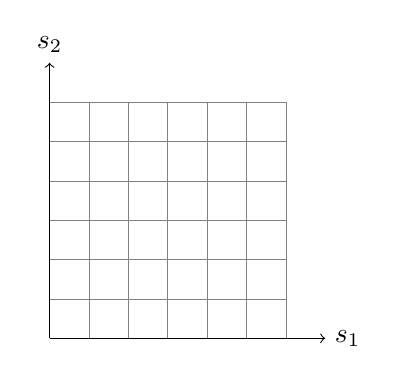
\begin{tikzpicture}[scale=1.0]
			\draw[step=0.5, gray, very thin] (0,0) grid (3,3);
			\draw[->] (0,0) -- (3.5,0) node[right] {$s_1$};
			\draw[->] (0,0) -- (0,3.5) node[above] {$s_2$};
		\end{tikzpicture}
	\end{center}
	\caption{Discretization for continuous state MDPs.}
	\label{fig:discretization}
	\end{figure}
	
	For example, a 2D state space $(s_1, s_2) \in \mathbb{R}^2$ is divided into grid cells, each representing a discrete state, allowing the application of standard MDP algorithms.
	
	\textbf{Advantages:}
	\begin{itemize}
		\item Simple to implement and effective for low-dimensional spaces ($n \leq 2$).
		\item Enables direct use of algorithms like value iteration and policy iteration.
	\end{itemize}
	
	\textbf{Disadvantages:}
	\begin{itemize}
		\item Suffers from the curse of dimensionality, as the number of states grows exponentially with $n$.
		\item Poor approximation for smooth value functions unless grid cells are very small, which increases computational cost.
	\end{itemize}
	
	Discretization is best suited for low-dimensional problems or when computational resources are not a limitation.
}

\Que{What is the main idea of value function approximation using a model or fitted value iteration?}
\Ans{
	Value function approximation replaces the need for discretization by representing the value function $V(s)$ as a parameterized function (e.g., linear or non-linear).
	
	\begin{itemize}
		\item \textbf{Using a Model:} With a known model $P_{sa}$, approximate $V(s)$ as $V(s) = \theta^\top \phi(s)$ and learn parameters $\theta$ by minimizing errors between predicted and observed values.
		\item \textbf{Fitted Value Iteration:} Iteratively refine $V(s)$ by sampling states $s^{(i)}$, computing target values $y^{(i)}$ using the Bellman equation, and fitting $V(s)$ to these targets via regression:
		\begin{equation}
			y^{(i)} = R(s^{(i)}) + \gamma \max_{a \in A} \mathbb{E}_{s' \sim P_{s^{(i)}a}}[V(s')].
		\end{equation}
	\end{itemize}
	
	This approach is well-suited for large, continuous state spaces where discretization becomes infeasible.
}



%\section{Recapitulation}
%- Key properties of probabilities: Positivity and total probability of 1.
%- Bayes theorem
%- Law of probability: $p(y|x) = p(x,y)p(x)$.
%- Marginalization: $p(x) = \int p(x,y)\,\mathrm{d}y$.
%- IID assumption: Identically and independently distributed. This makes $p(x^{(1)},\dots,x^{(m)})  = \prod_{i=1}^{m}p(x^{(i)})$.
%- Maximum a posteriori optimization.
%- Maximum likelihood optimization.

\end{document}
